\begin{appendices}
	\newgeometry{top=0.7in,bottom=0.7in,left=1in,right=1in}

	\chapter{Simulated Group Topologies}
	\section{K-Nearest Neighbour Clustering}
	\label{appendix:knn}
	\begin{figure}
		\centering
		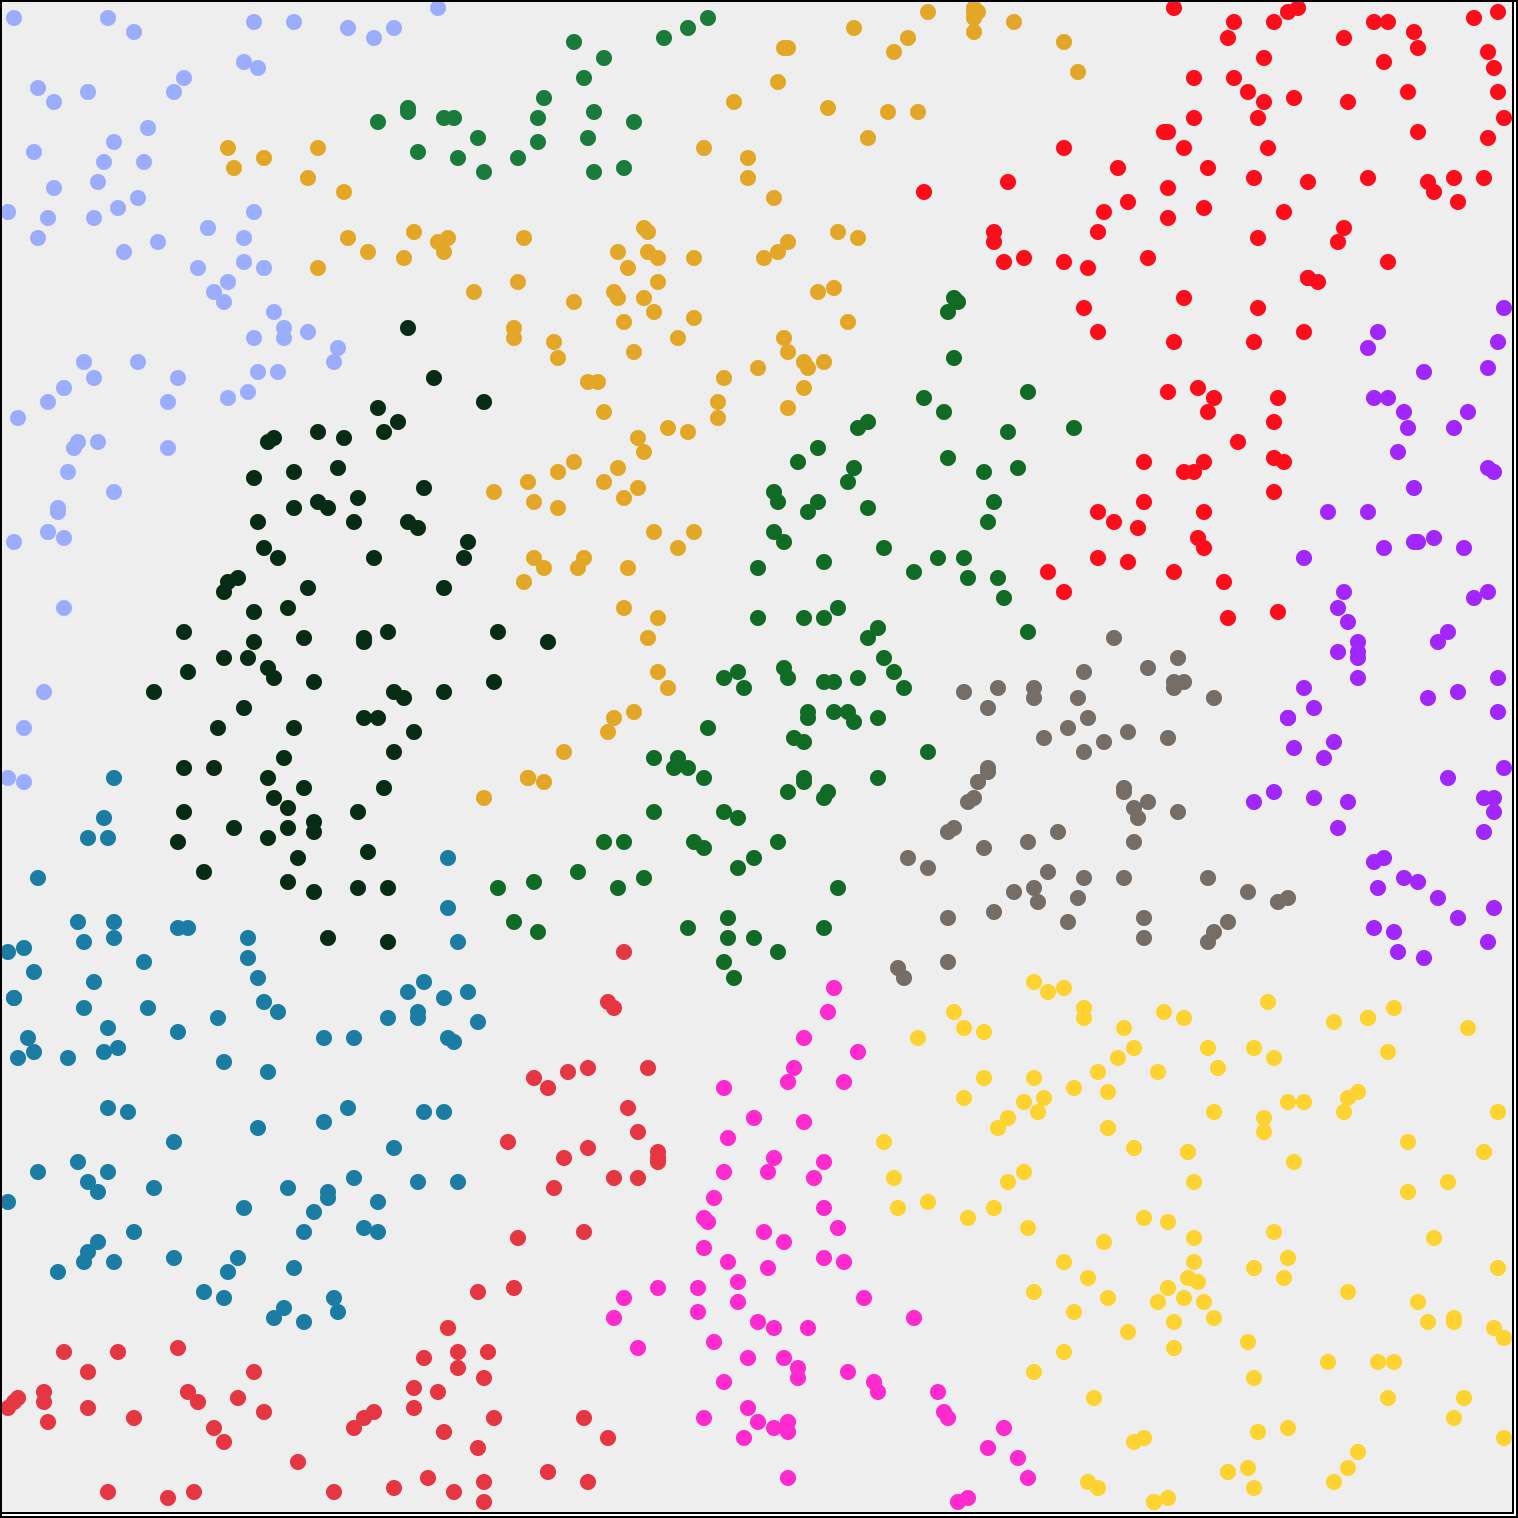
\includegraphics[width=11cm]{Images/computations/BASIC500x500_1000n.jpg}
		\caption{Uniform distribution, 500x500, 1000 nodes}
	\end{figure}

	\begin{figure}[H]
		\centering
		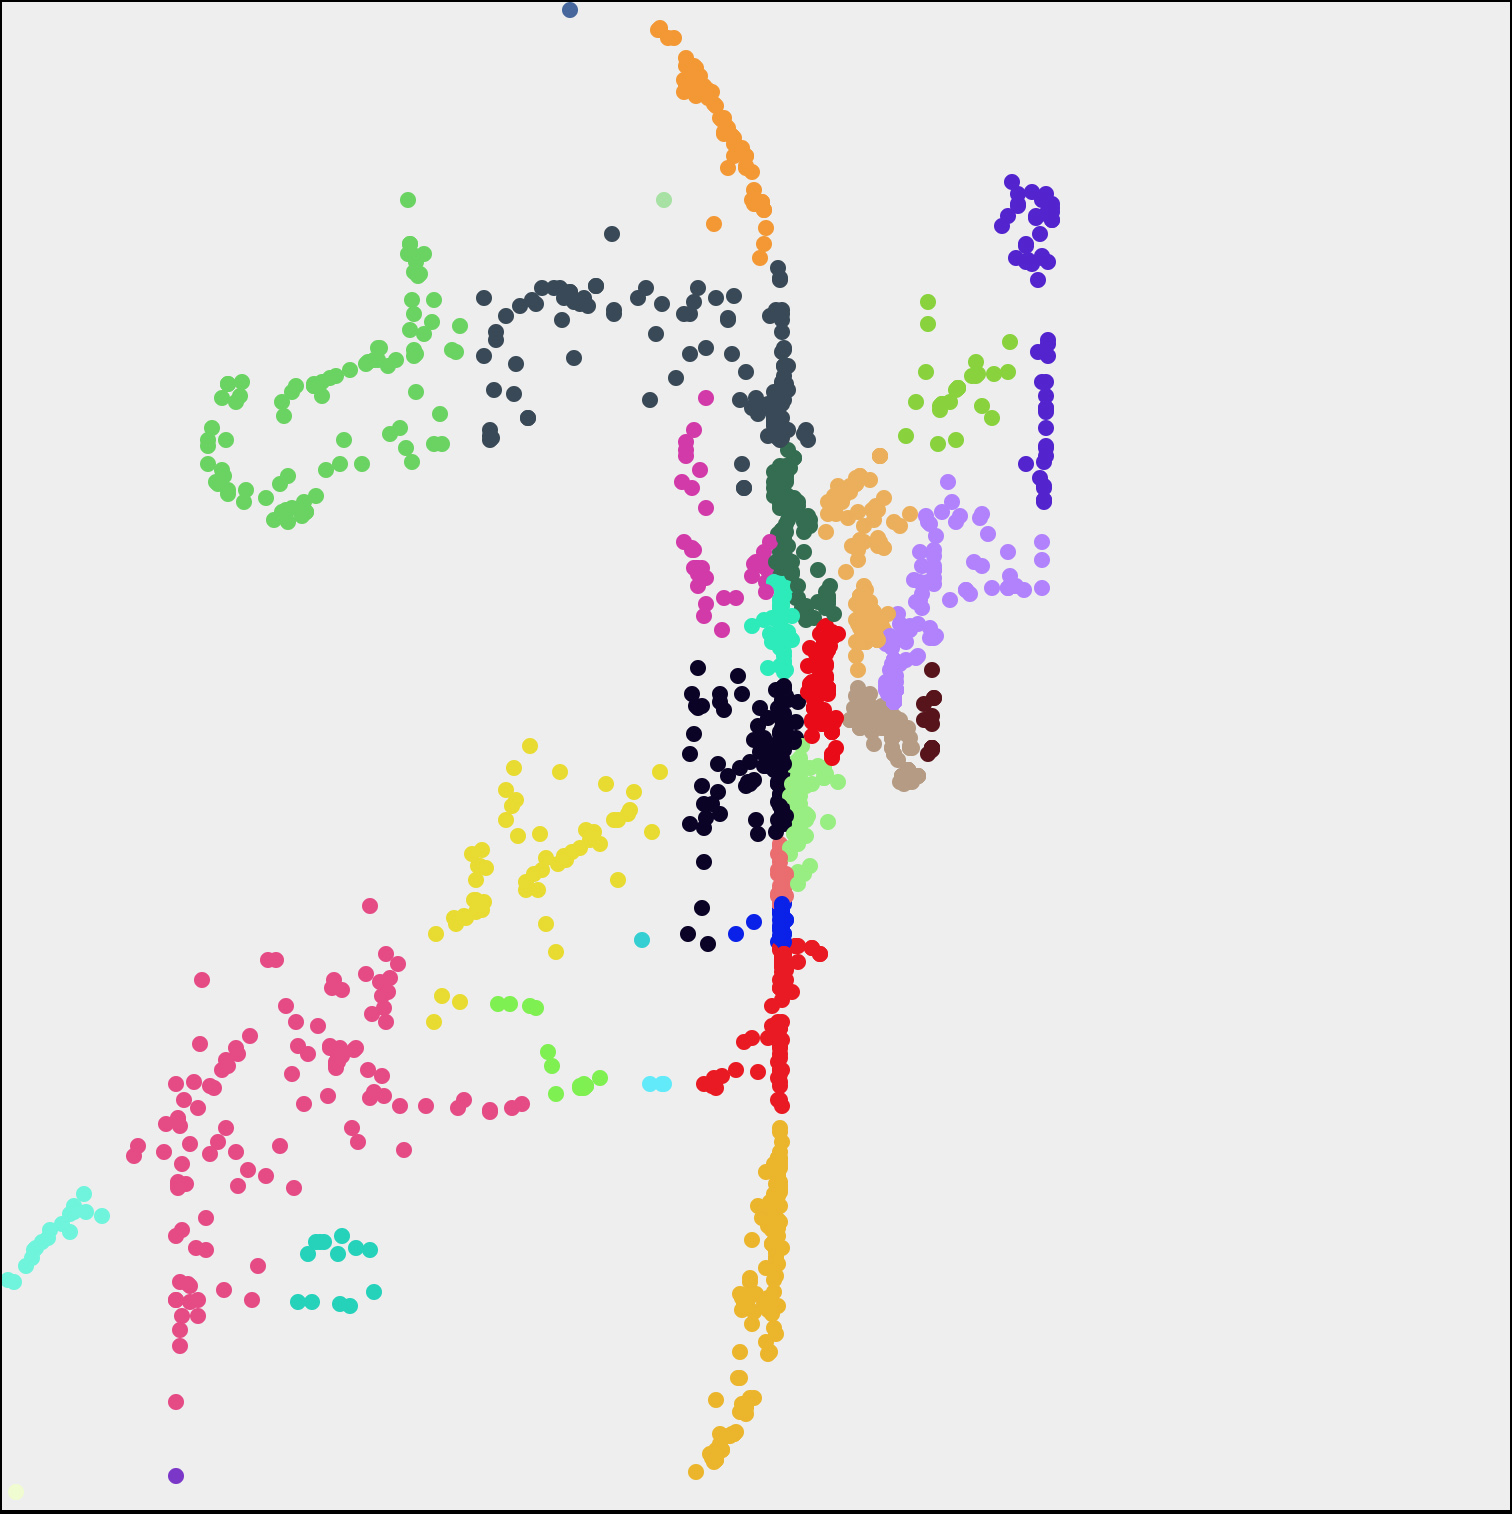
\includegraphics[width=11cm]{Images/computations/BASICForks.jpg}
		\caption{Forks, Washington, USA}
	\end{figure}

	\begin{figure}
		\centering
		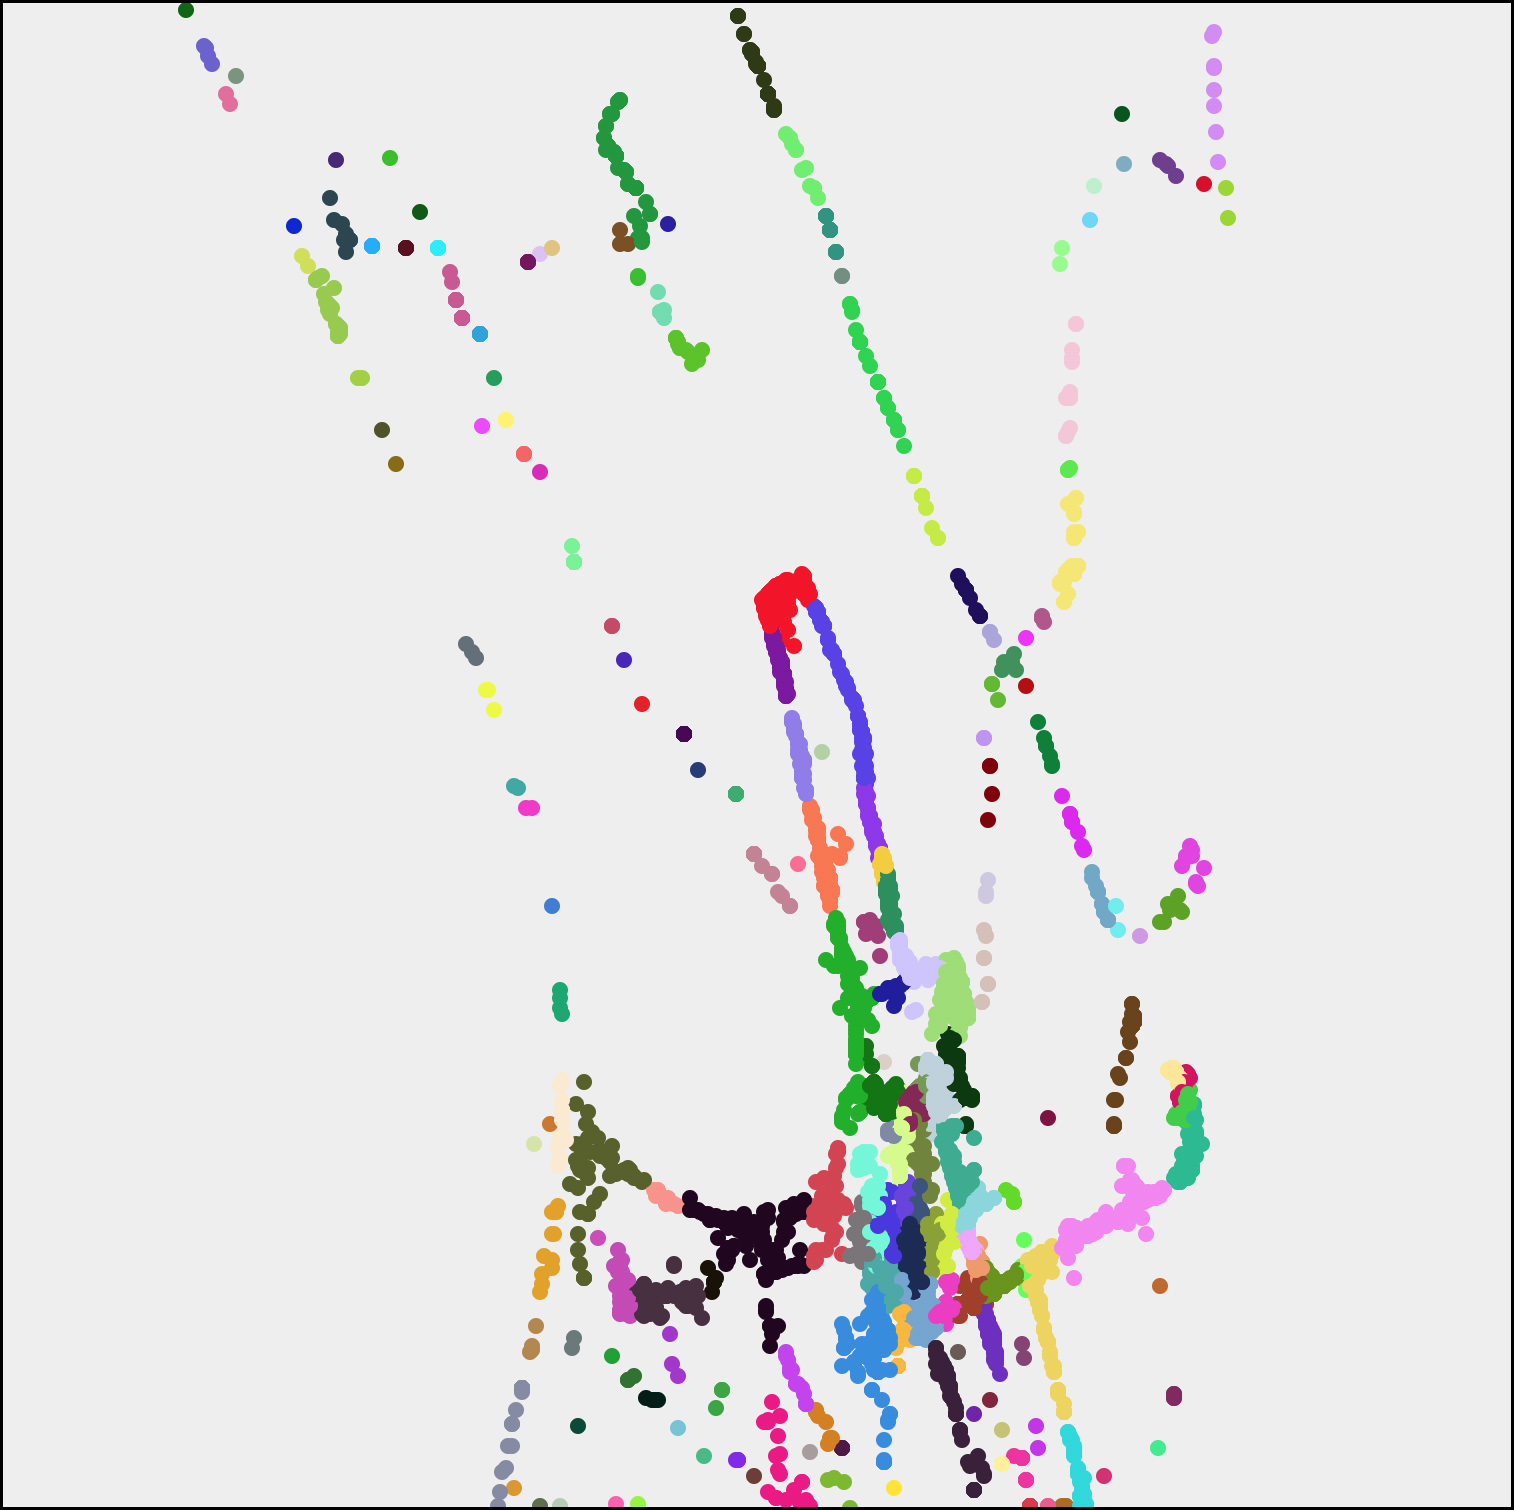
\includegraphics[width=11cm]{Images/computations/BASICLillehammer.jpg}
		\caption{Lillehammer, Norway}
	\end{figure}

	\begin{figure}[H]
		\centering
		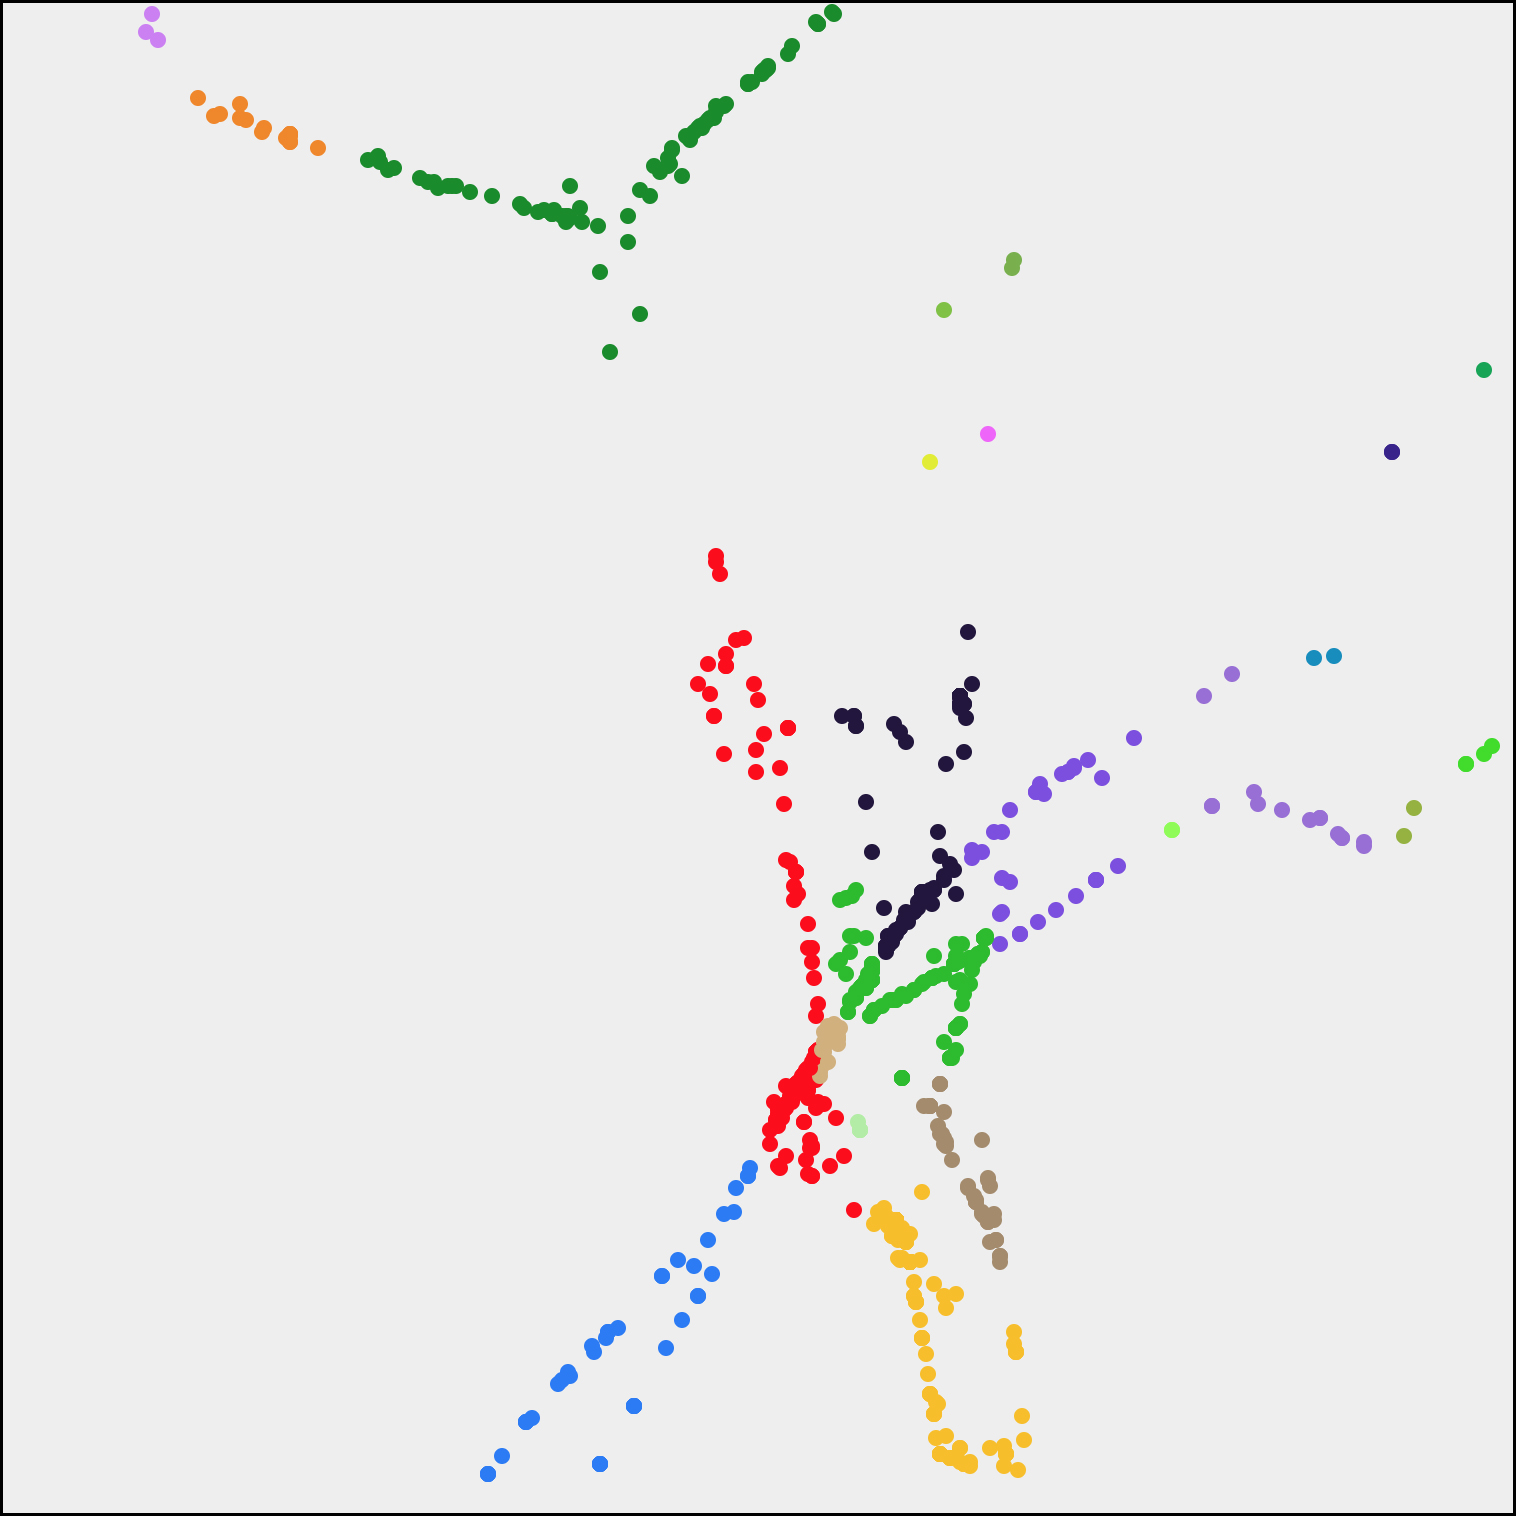
\includegraphics[width=11cm]{Images/computations/BASICTynset.jpg}
		\caption{Tynset, Norway}
	\end{figure}
	






		%	\qquad
		%	\\subfloat[Forks]{{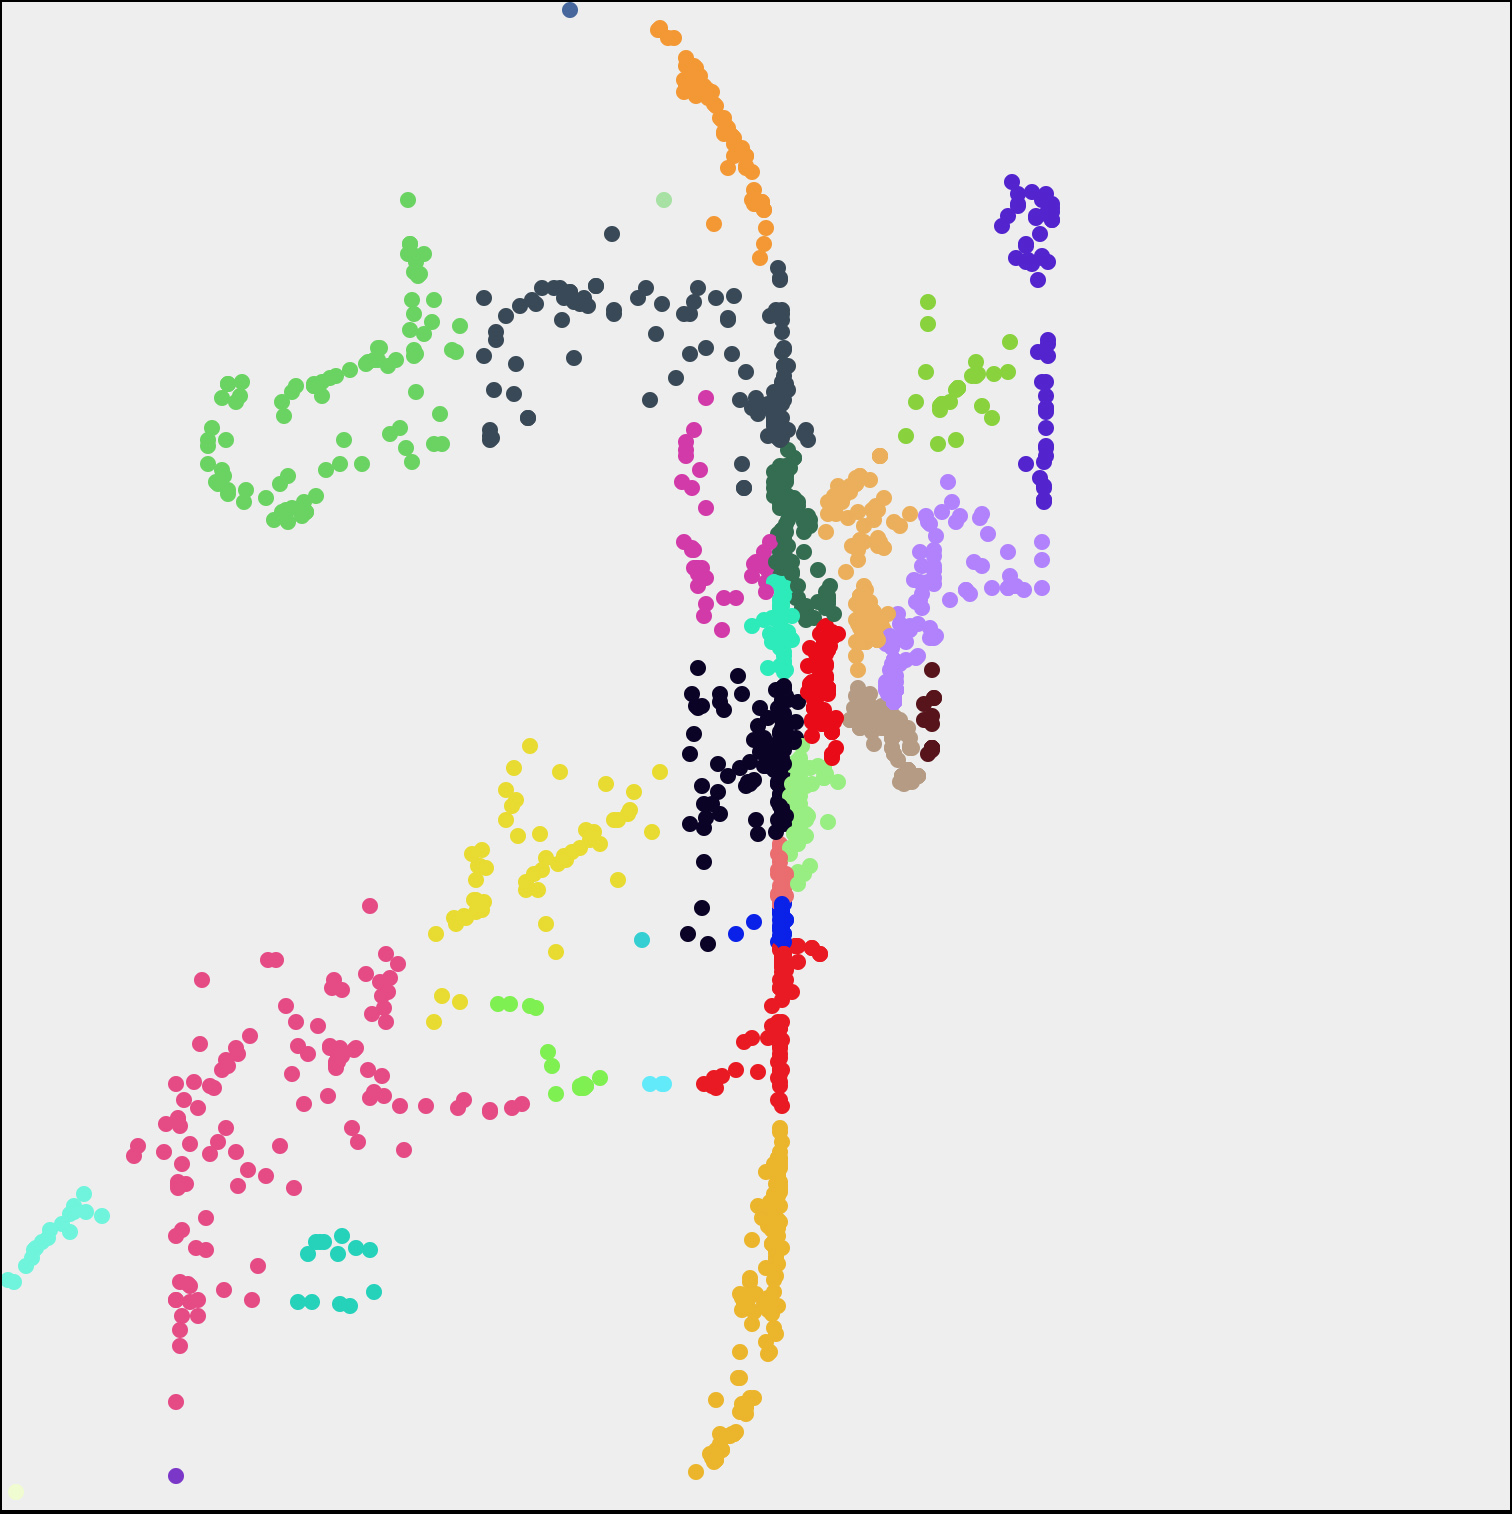
\includegraphics[width=6cm]{Images/computations/BASICForks.jpg} }}%
		%	\\newline
		%	\\subfloat[Lillehammer]{{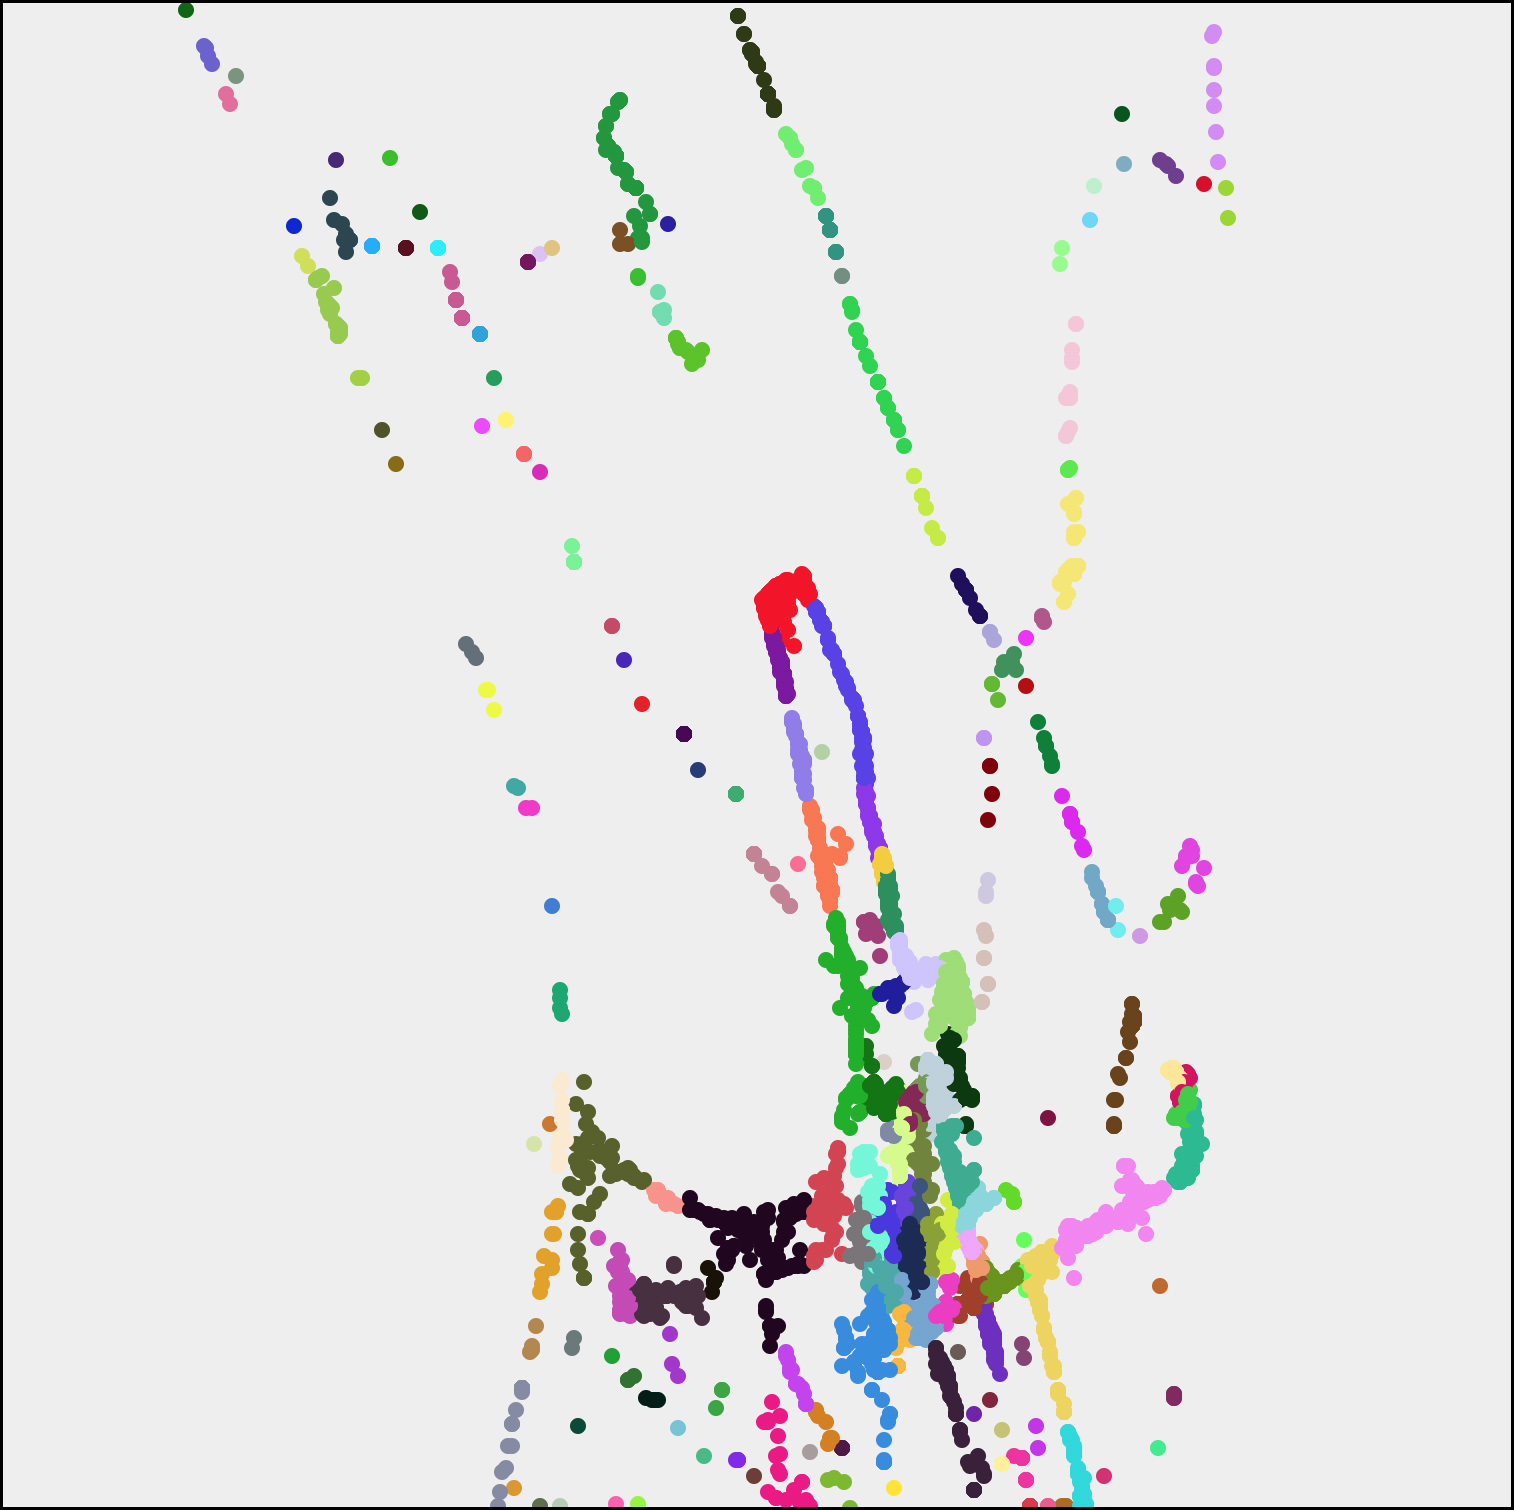
\includegraphics[width=6cm]{Images/computations/BASICLillehammer.jpg} }}%
		%	\\qquad
		%	\\subfloat[Tynset]{{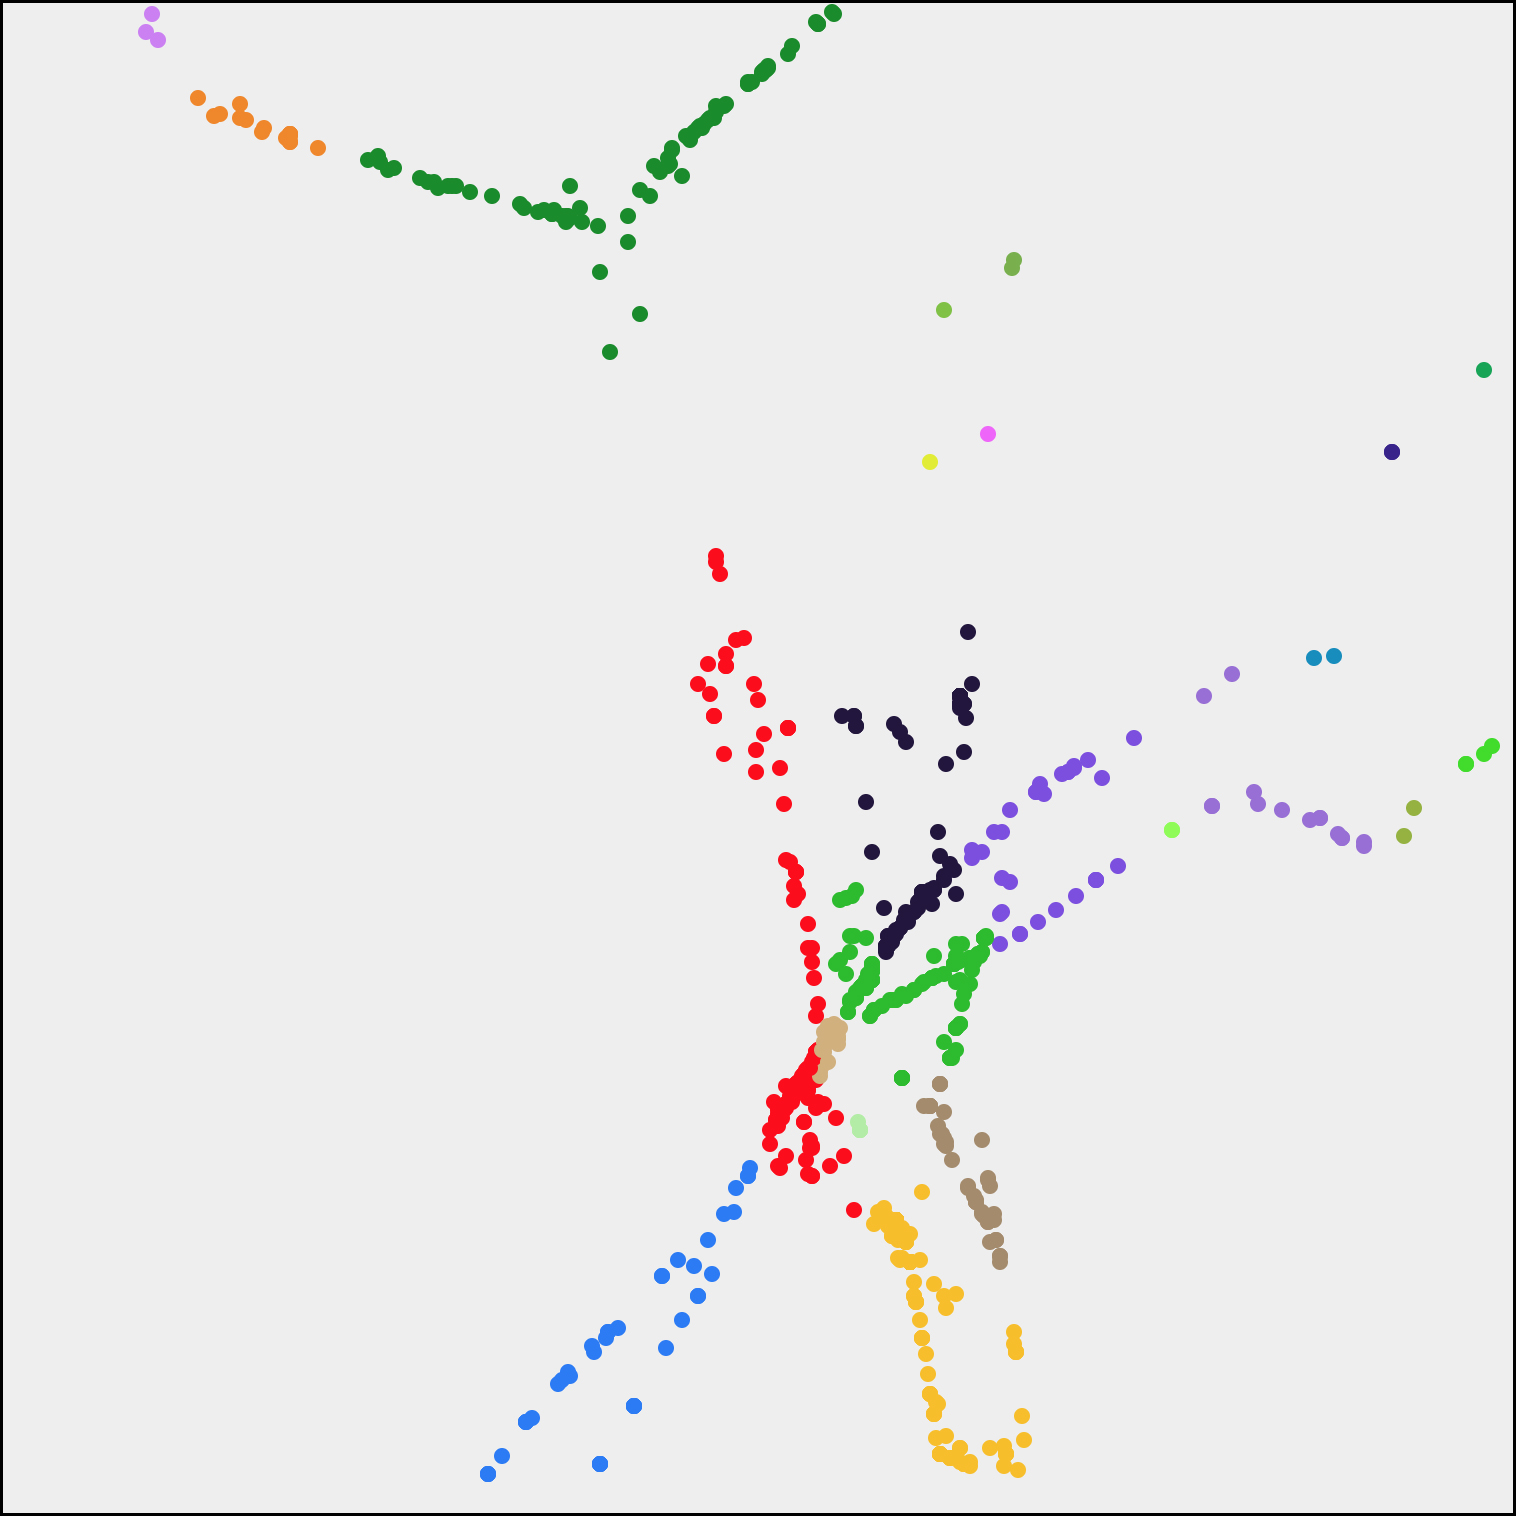
\includegraphics[width=6cm]{Images/computations/BASICTynset.jpg} }}%
		%	\\caption{K-Nearest Neighbour Clustering on different topologies}%
		%	\\label{fig:knearest}%


	\section{K-means Split}
	\label{appendix:kmeanssplit}
	\begin{figure}
		\centering
		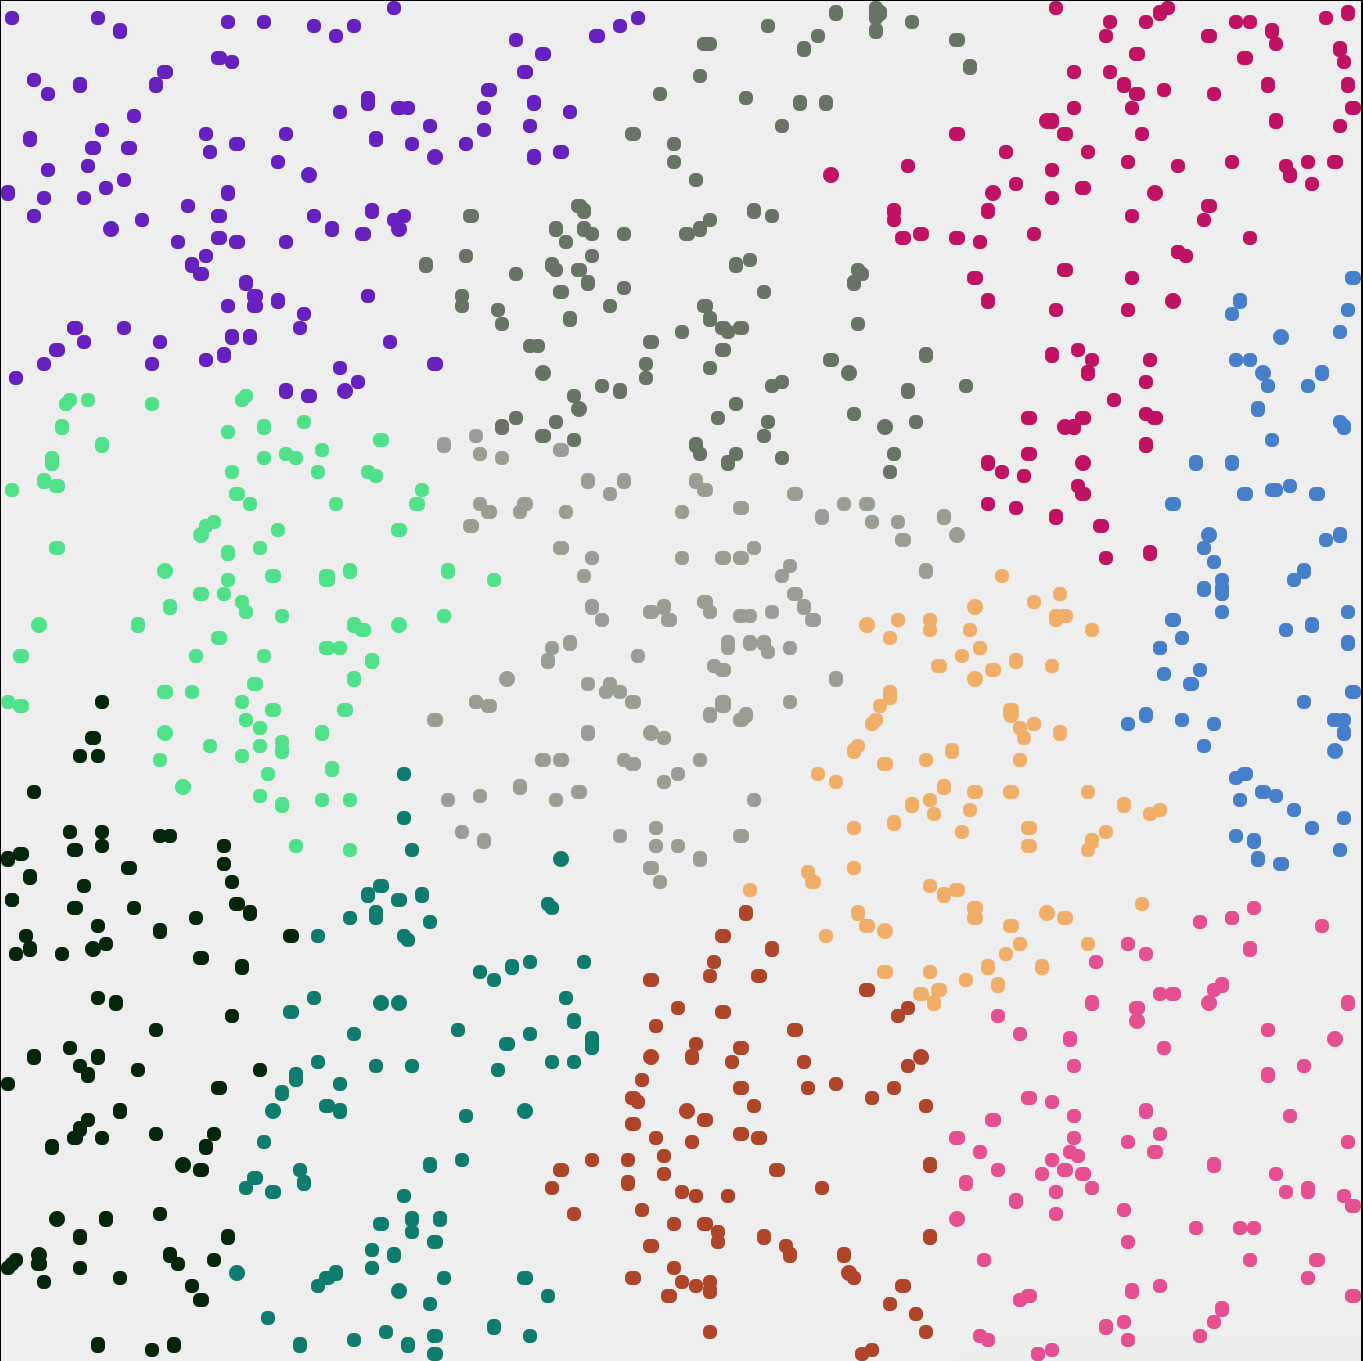
\includegraphics[width=11cm]{Images/computations/KMEANS500x500_1000n.jpg}
		\caption{Uniform distribution, 500x500, 1000 nodes}
	\end{figure}

	\begin{figure}[H]
		\centering
		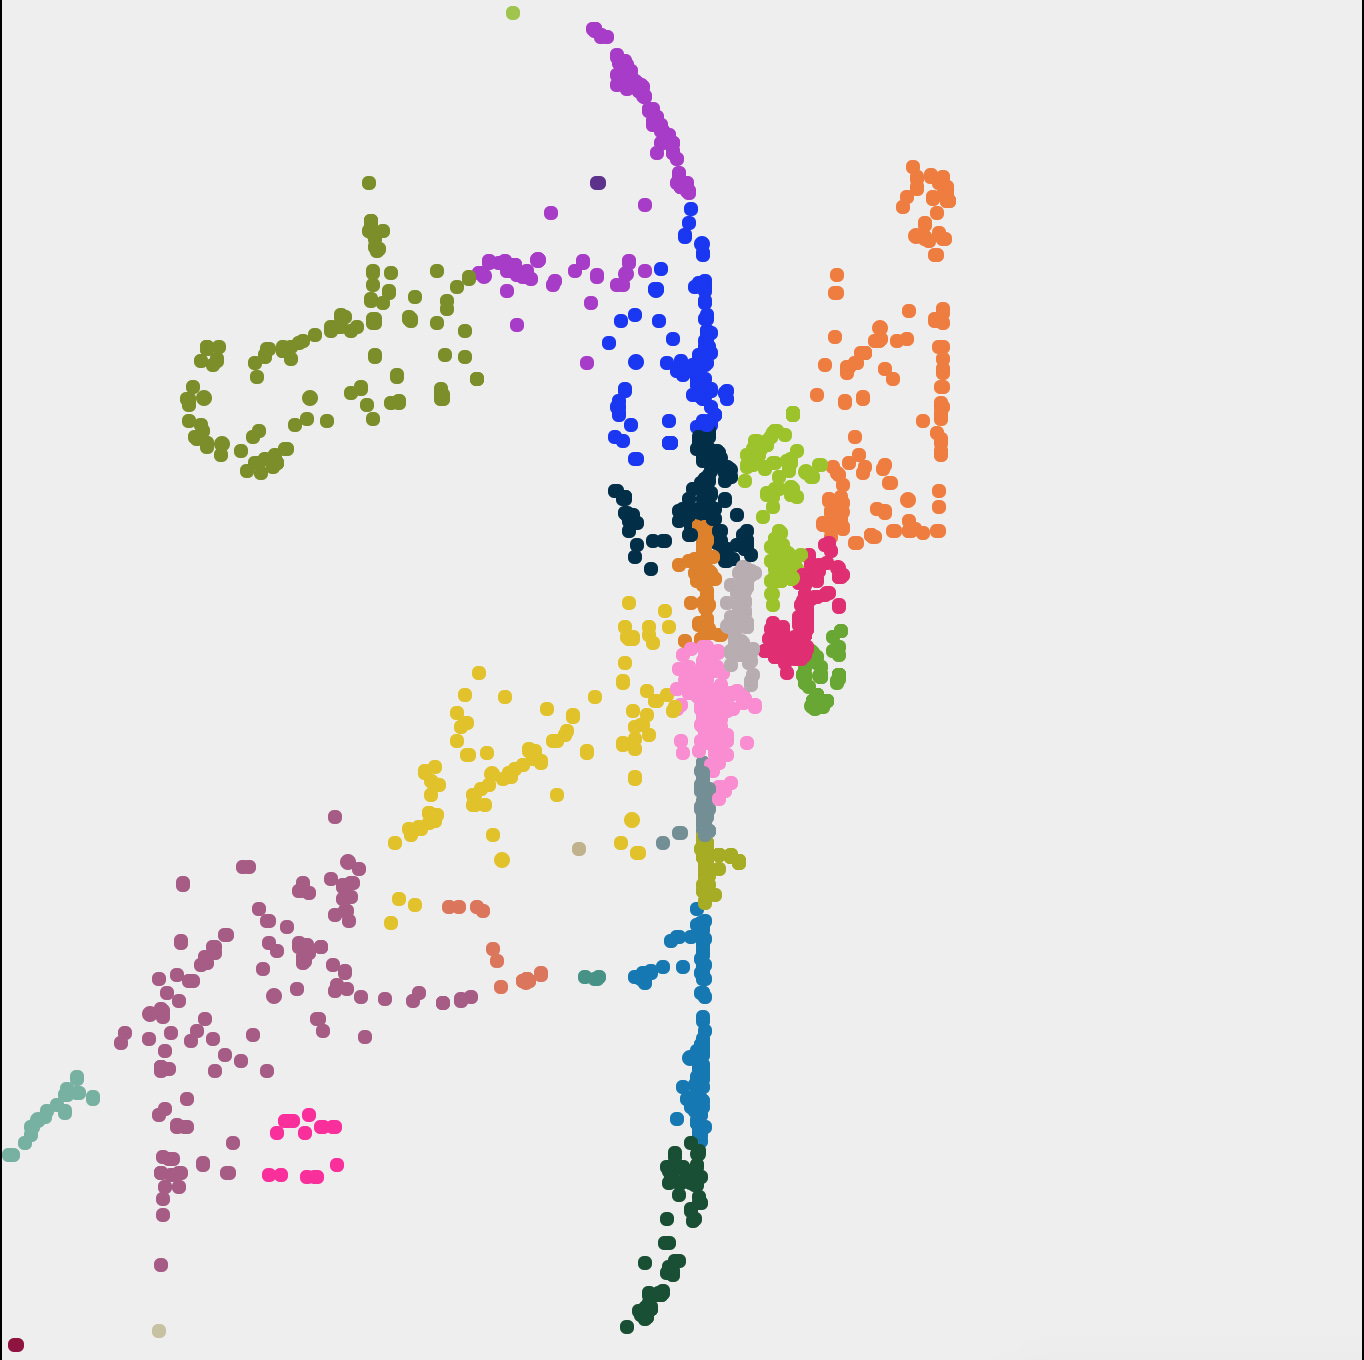
\includegraphics[width=11cm]{Images/computations/KMEANSForks.jpg}
		\caption{Forks, Washington, USA}
	\end{figure}

	\begin{figure}
		\centering
		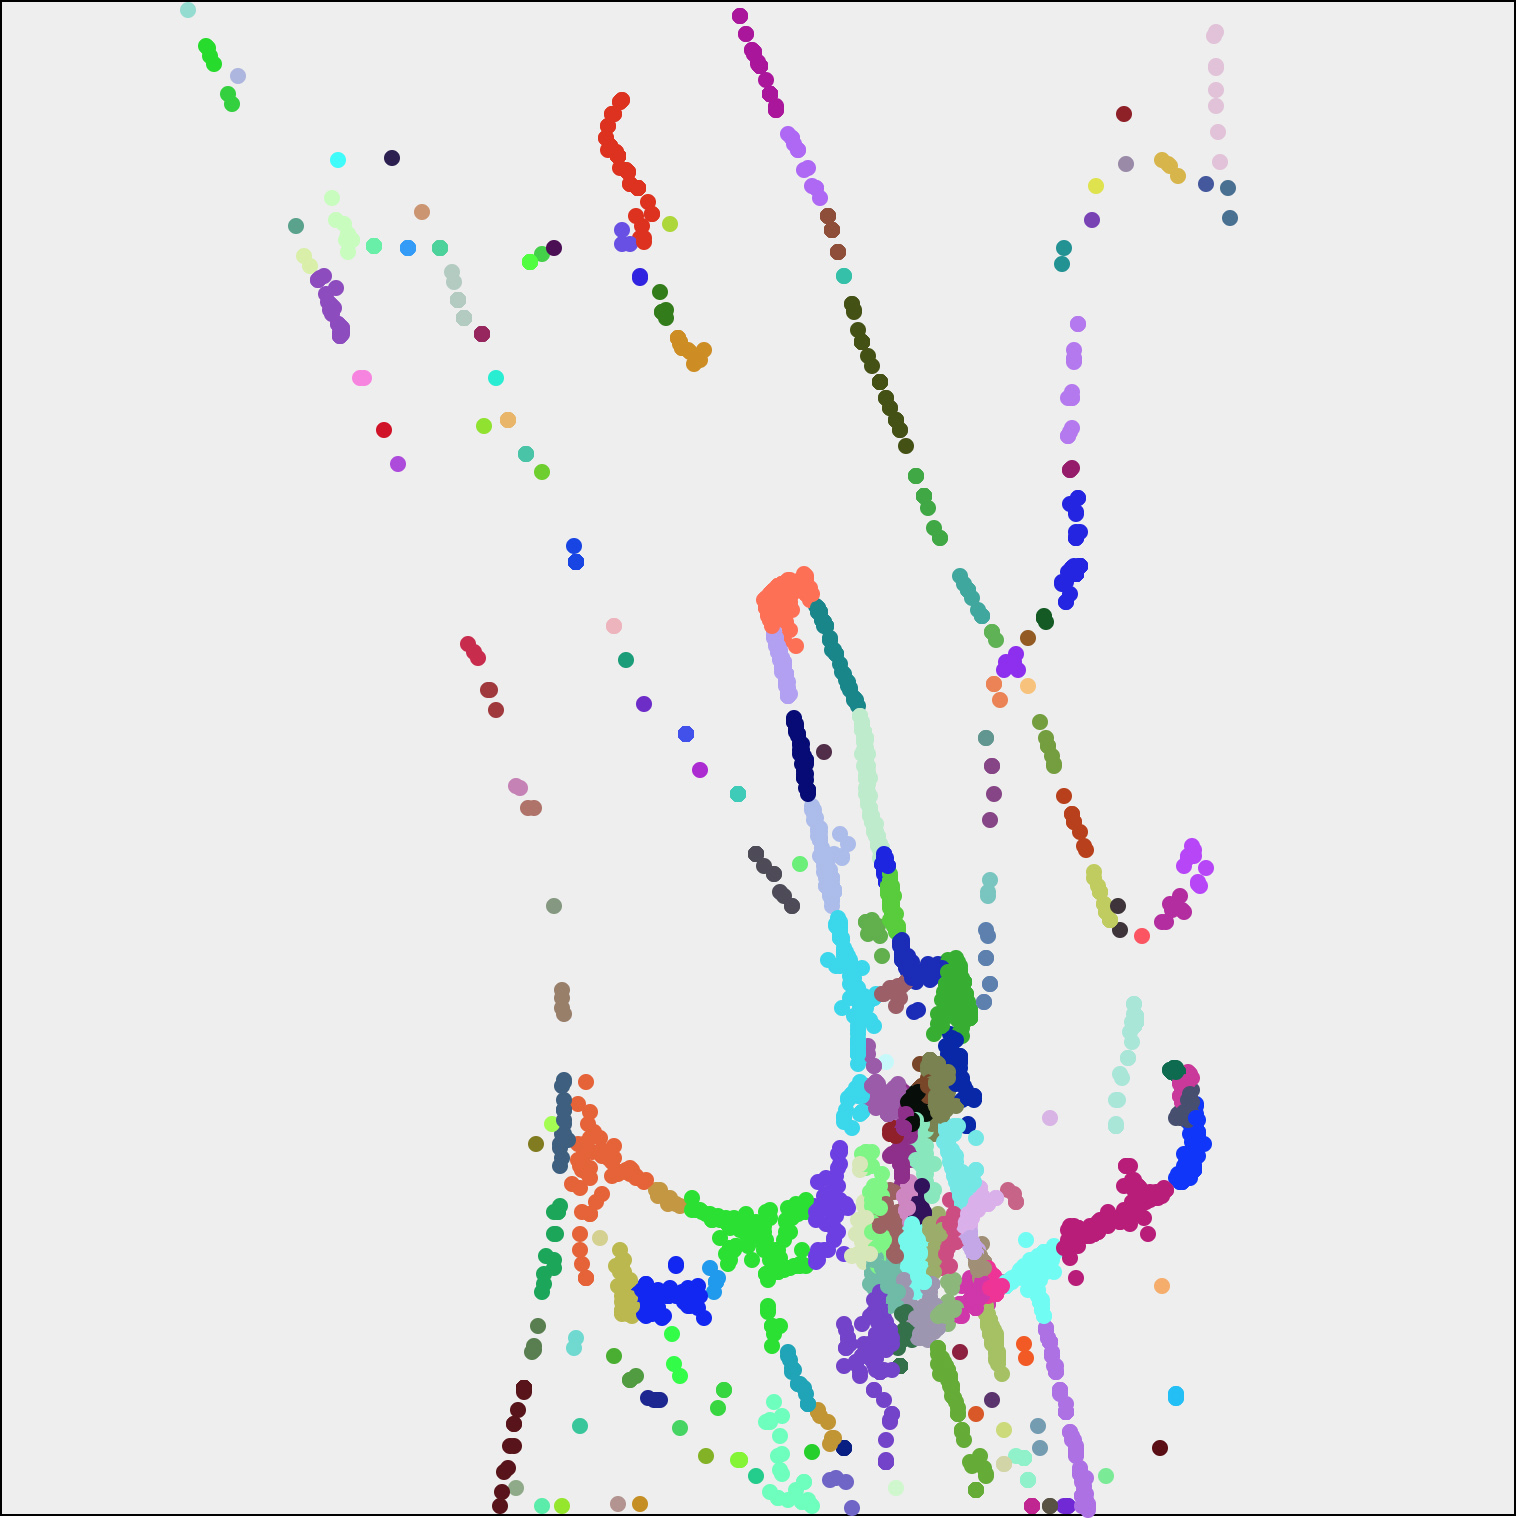
\includegraphics[width=11cm]{Images/computations/KMEANSLillehammer.jpg}
		\caption{Lillehammer, Norway}
	\end{figure}

	\begin{figure}[H]
		\centering
		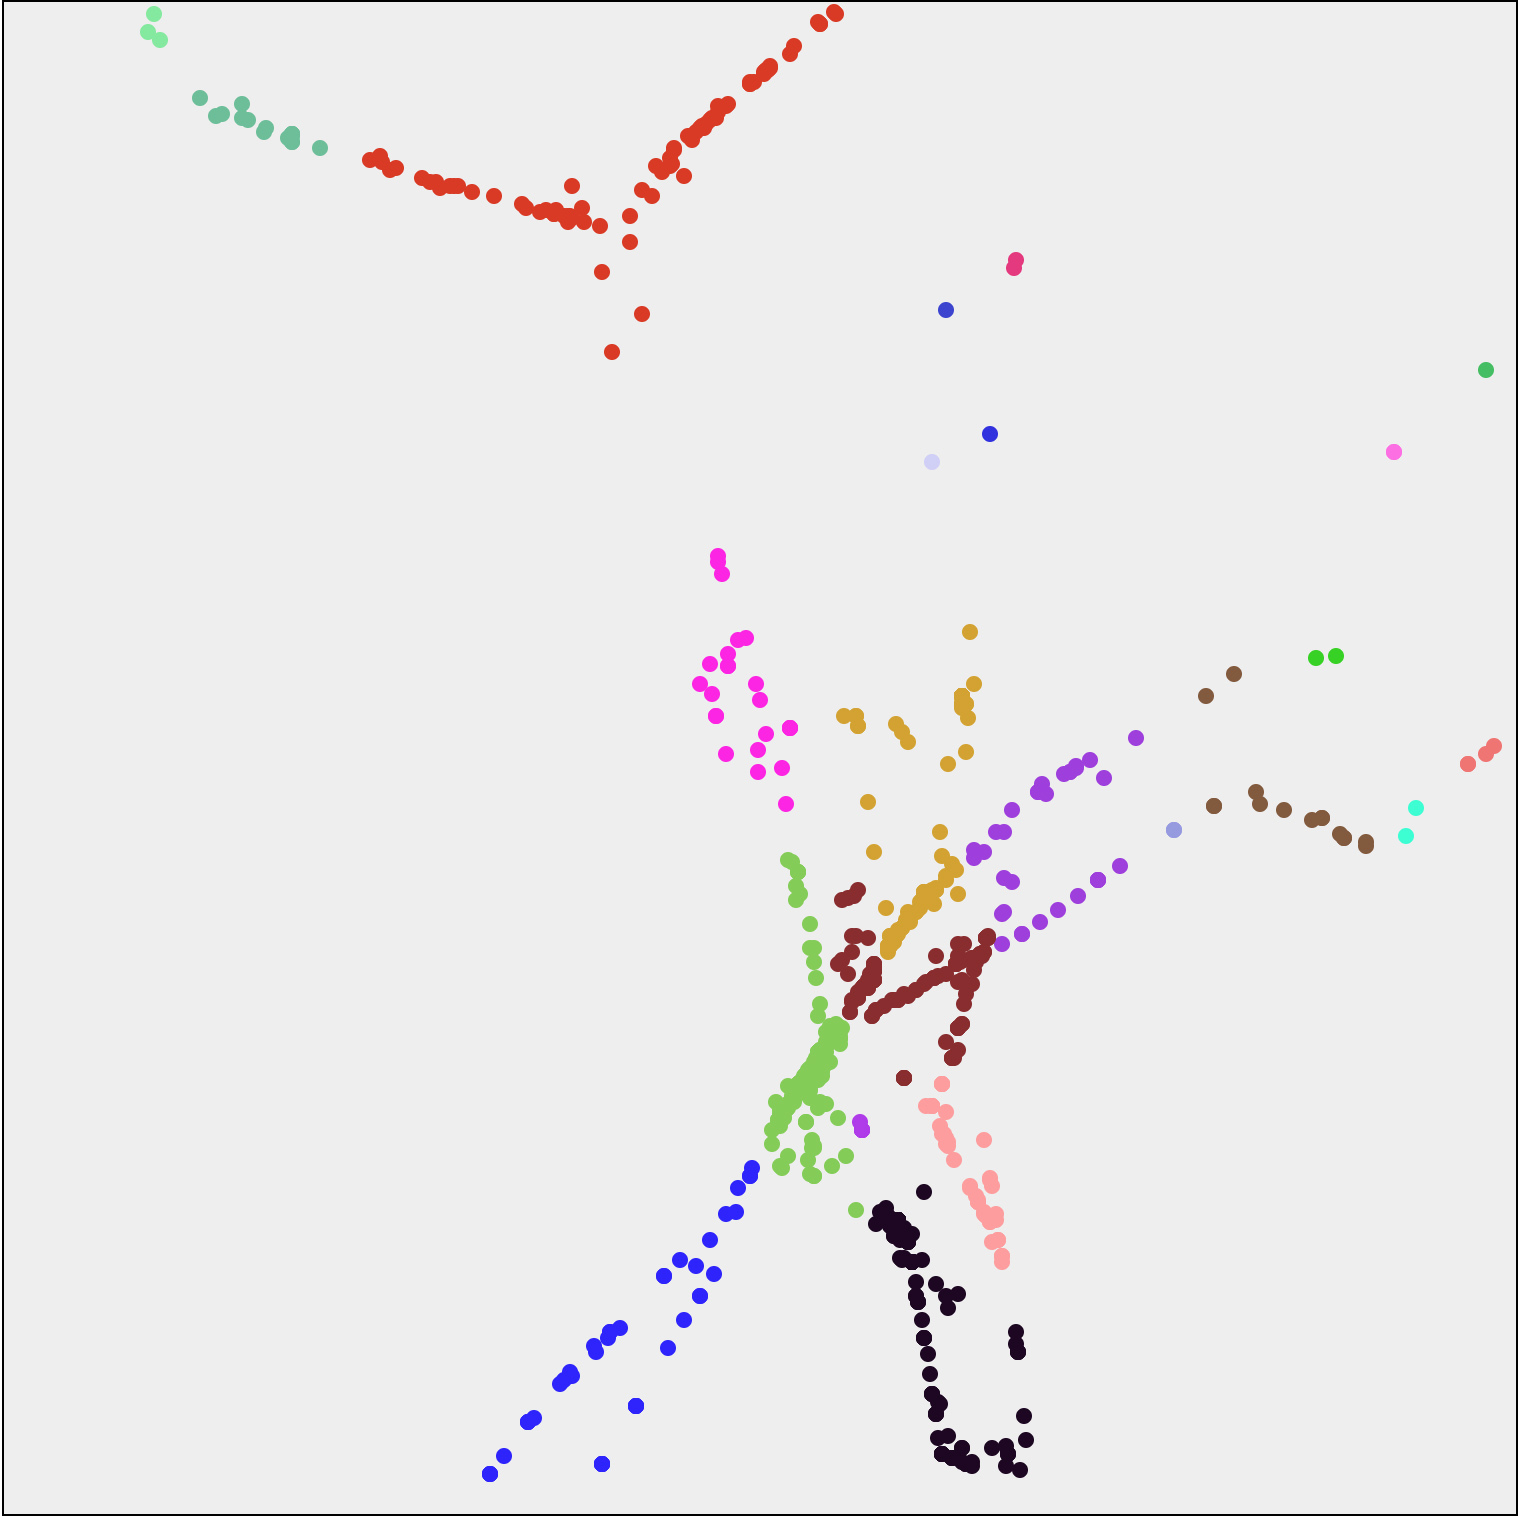
\includegraphics[width=11cm]{Images/computations/KMEANSTynset.jpg}
		\caption{Tynset, Norway}
	\end{figure}



	\section{Original Minimum Cut Split}
	\label{appendix:mincutsplitone}
	\begin{figure}
		\centering
		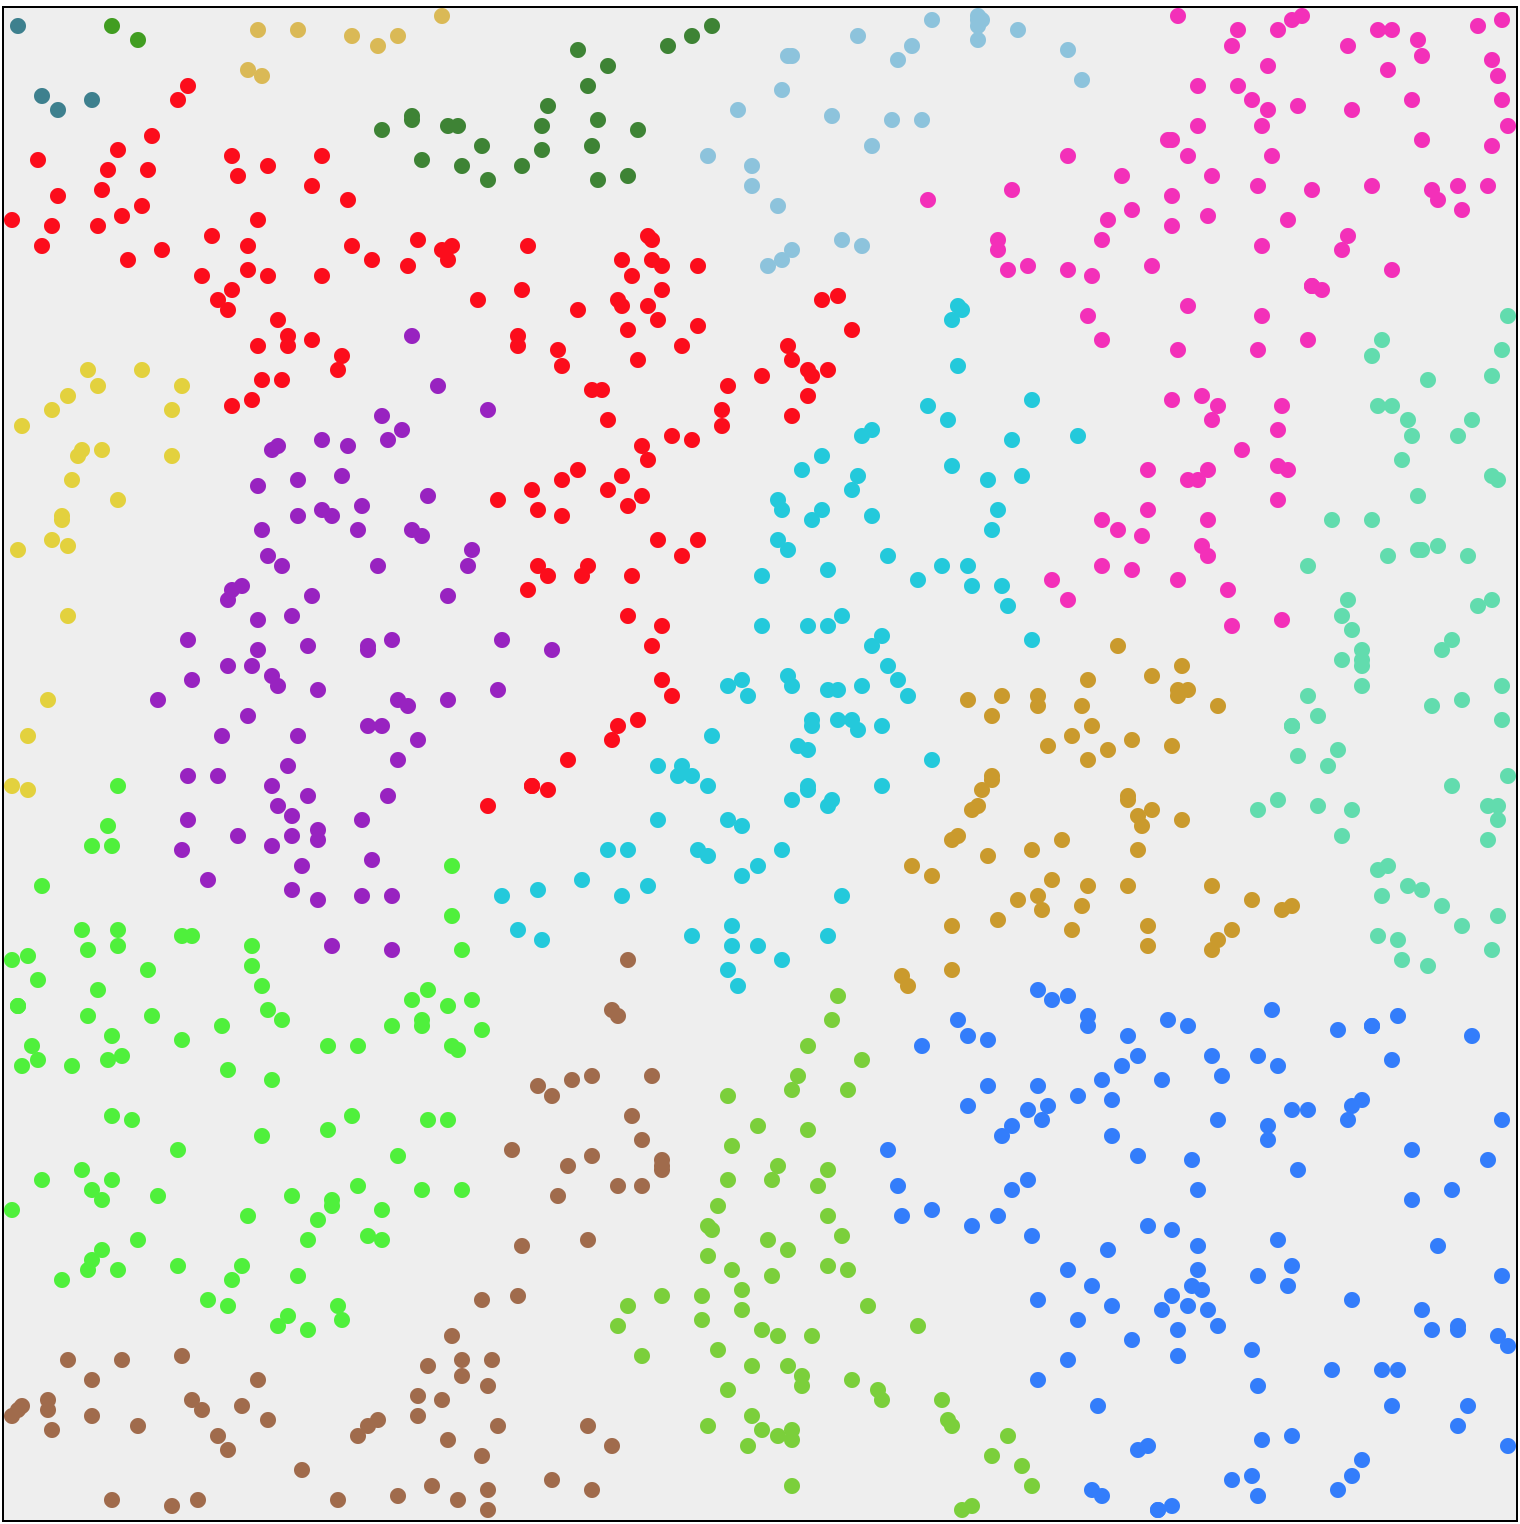
\includegraphics[width=11cm]{Images/computations/MINCUT500_500.png}
		\caption{Uniform distribution, 500x500, 1000 nodes}
	\end{figure}

	\begin{figure}[H]
		\centering
		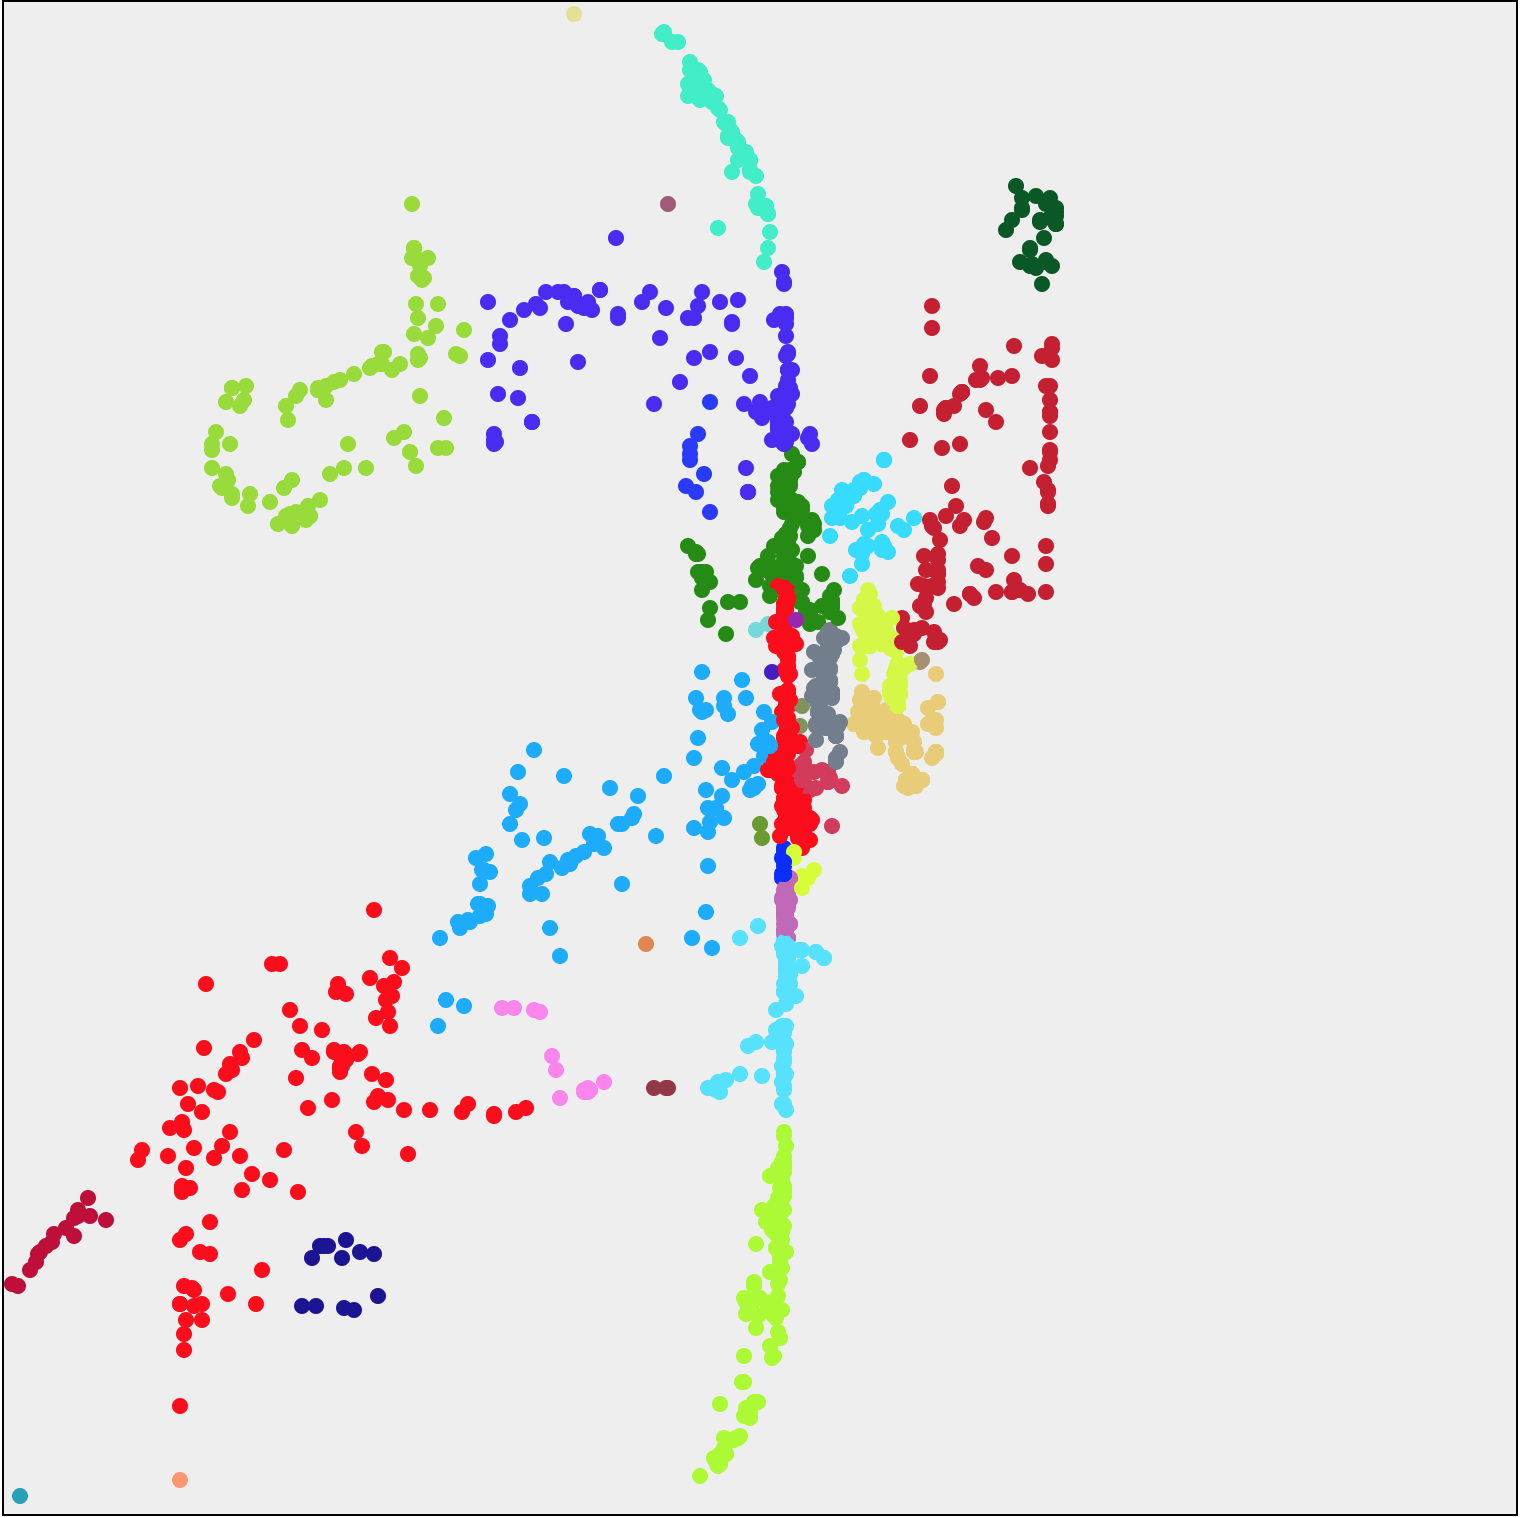
\includegraphics[width=11cm]{Images/computations/MINCUT_FORKS.png}
		\caption{Forks, Washington, USA}
	\end{figure}

	\begin{figure}
		\centering
		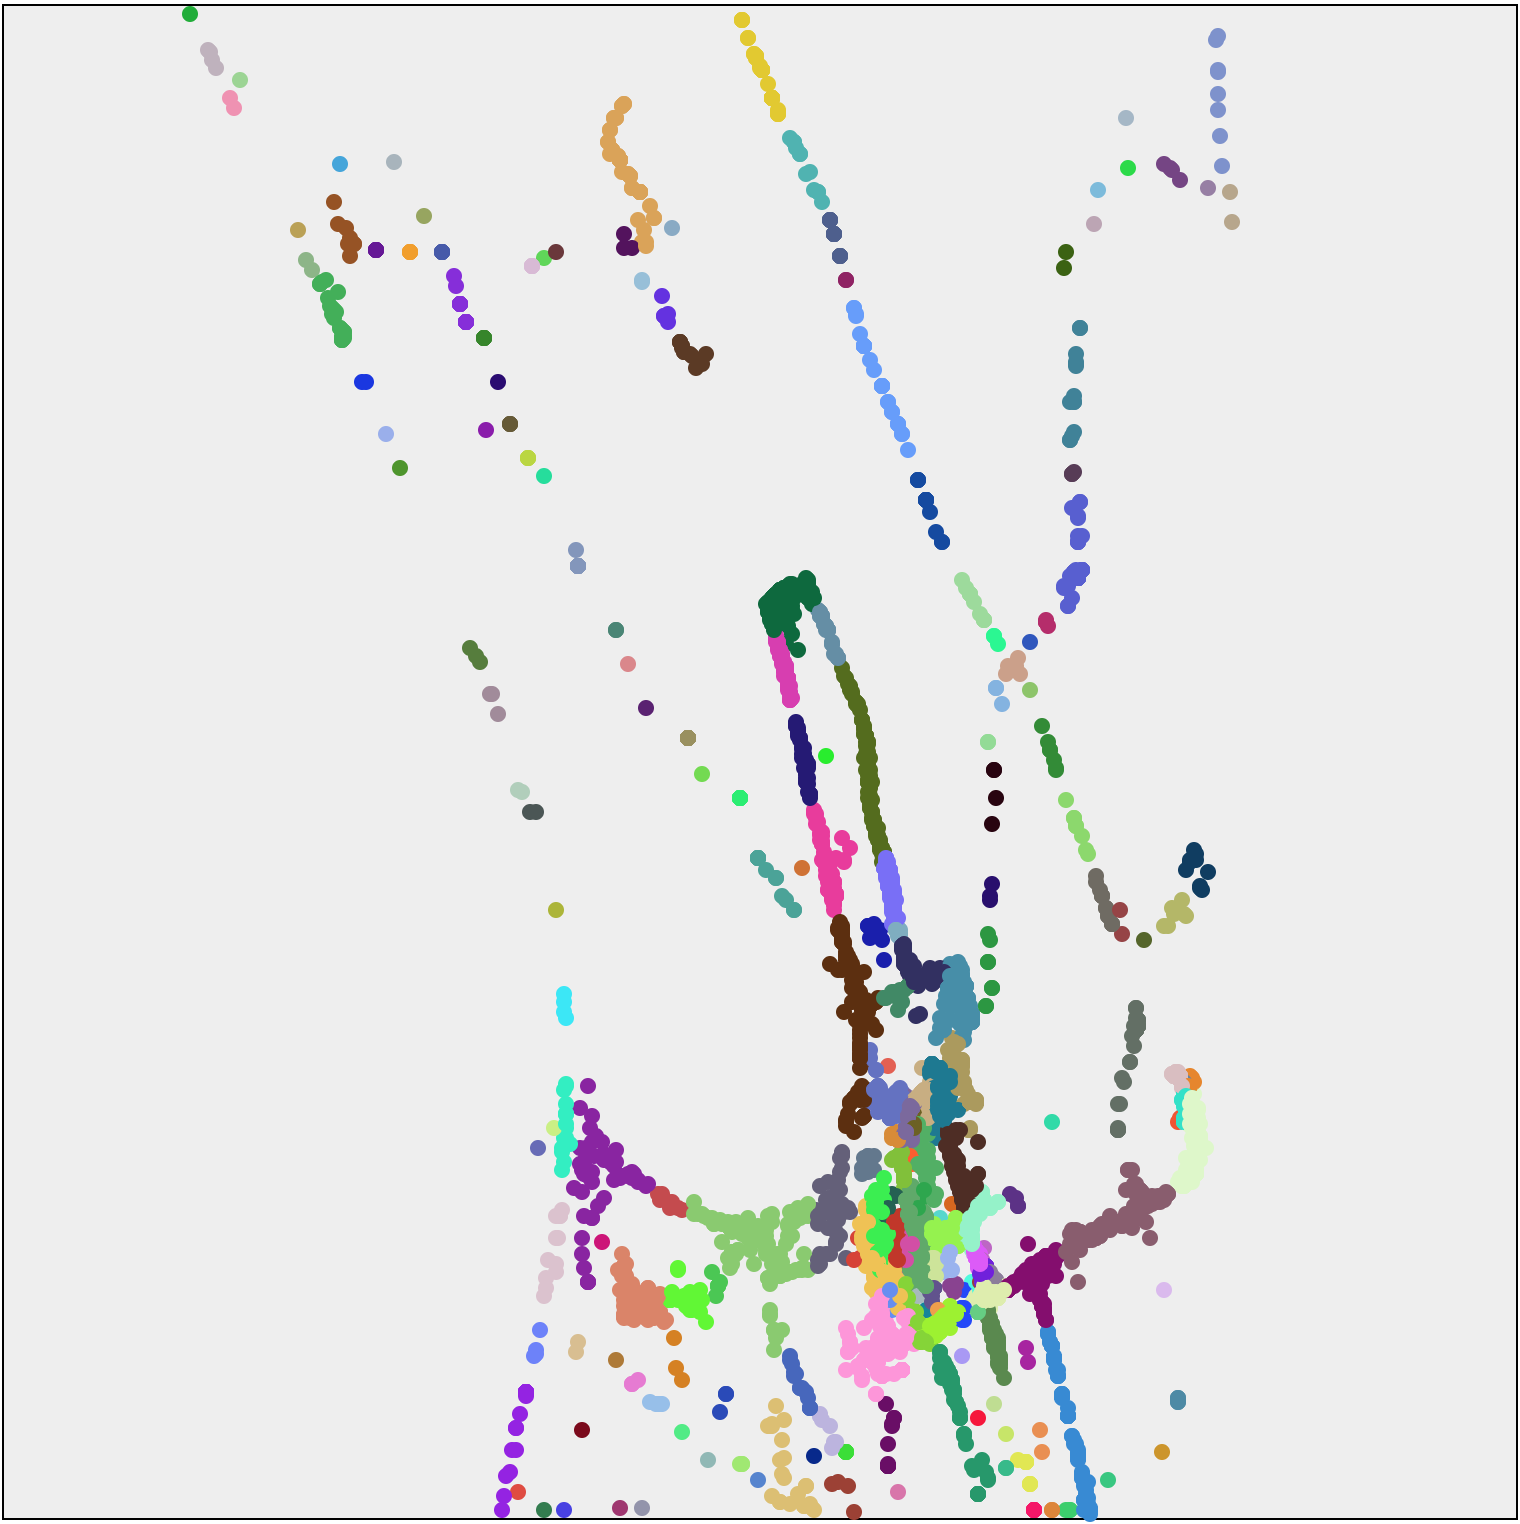
\includegraphics[width=11cm]{Images/computations/MINCUT_LILLEHAMMER.png}
		\caption{Lillehammer, Norway}
	\end{figure}

	\begin{figure}[H]
		\centering
		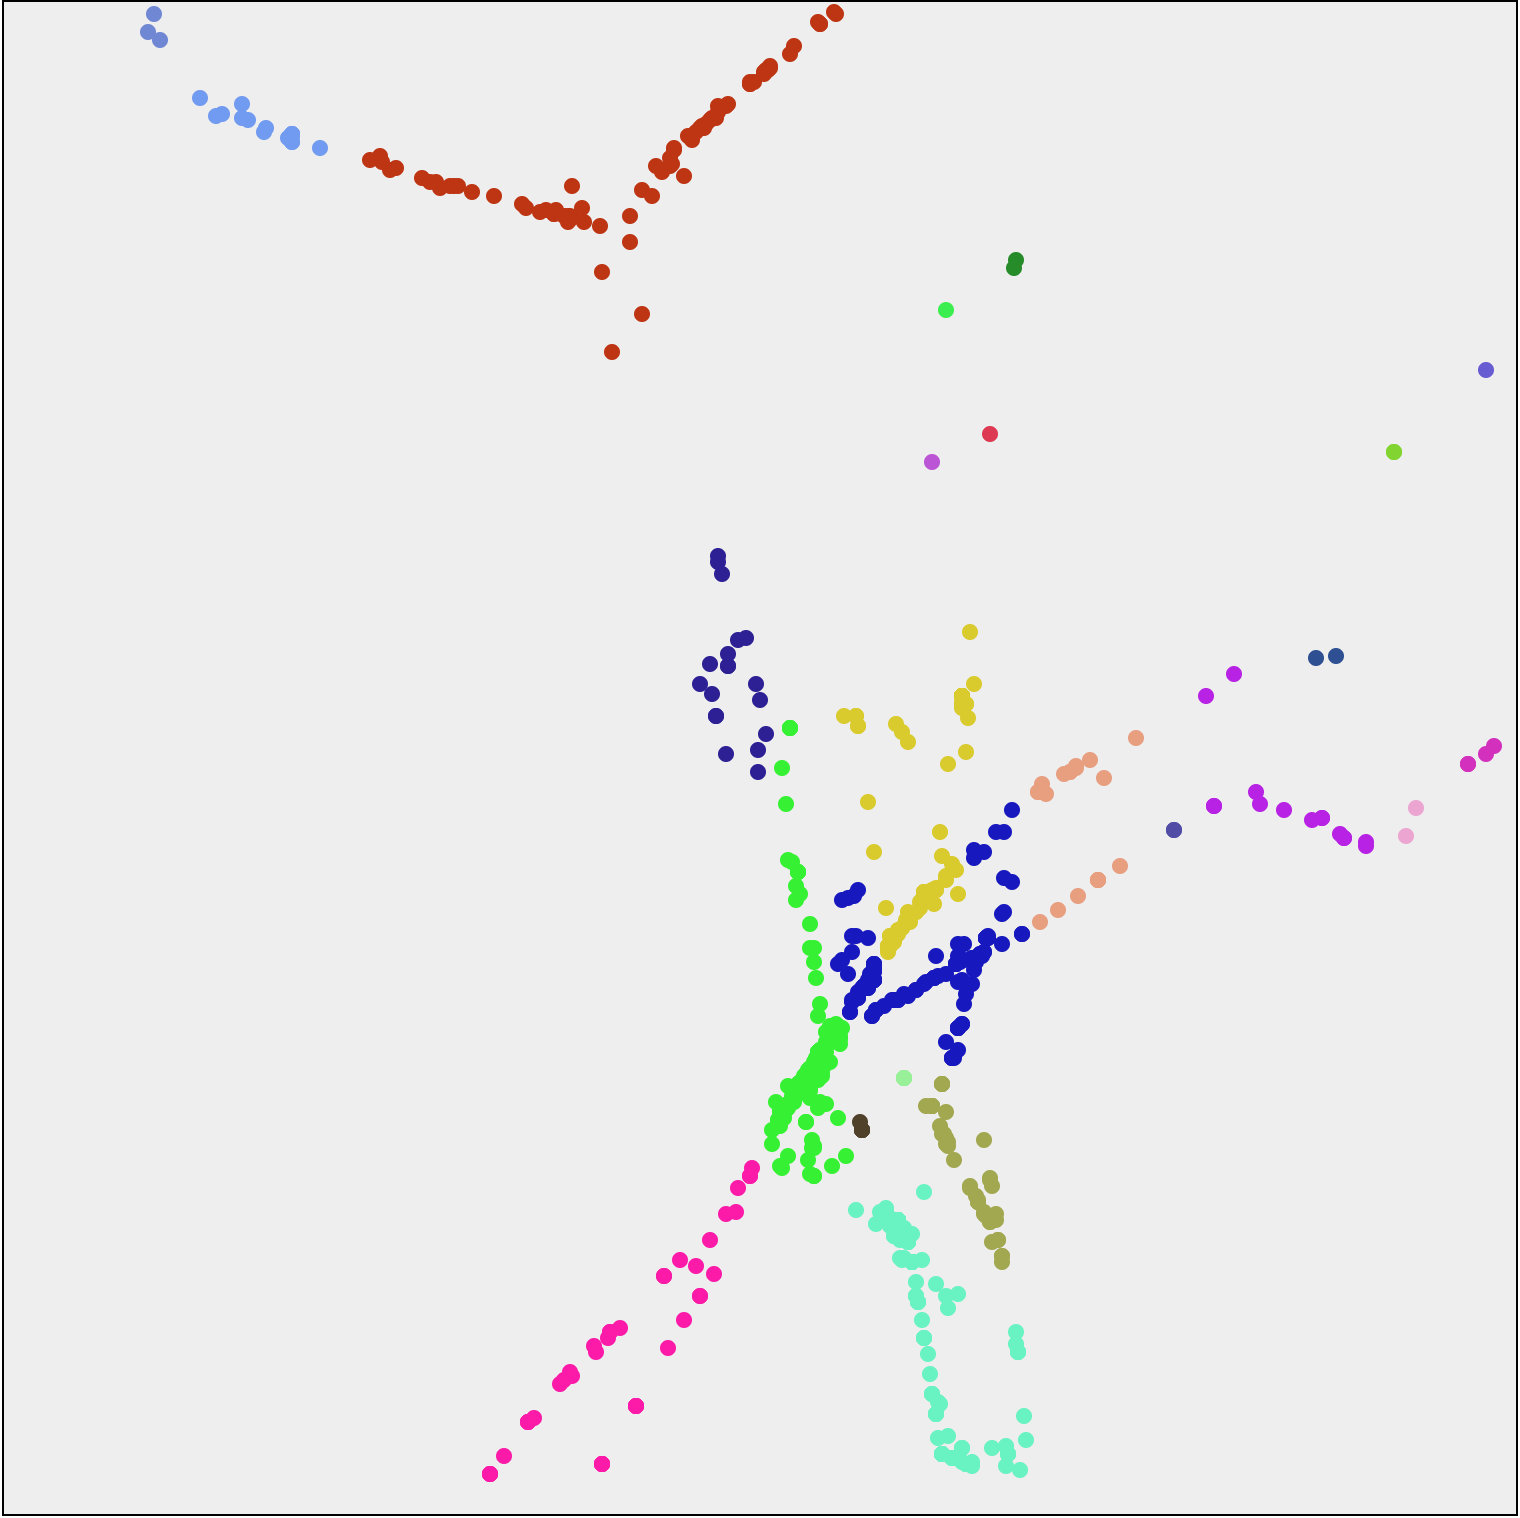
\includegraphics[width=11cm]{Images/computations/MINCUT_TYNSET.png}
		\caption{Tynset, Norway}
	\end{figure}


	\section{Re-evaluated Minimum Cut Split}
	\label{appendix:mincutsplittwo}
	\begin{figure}
		\centering
		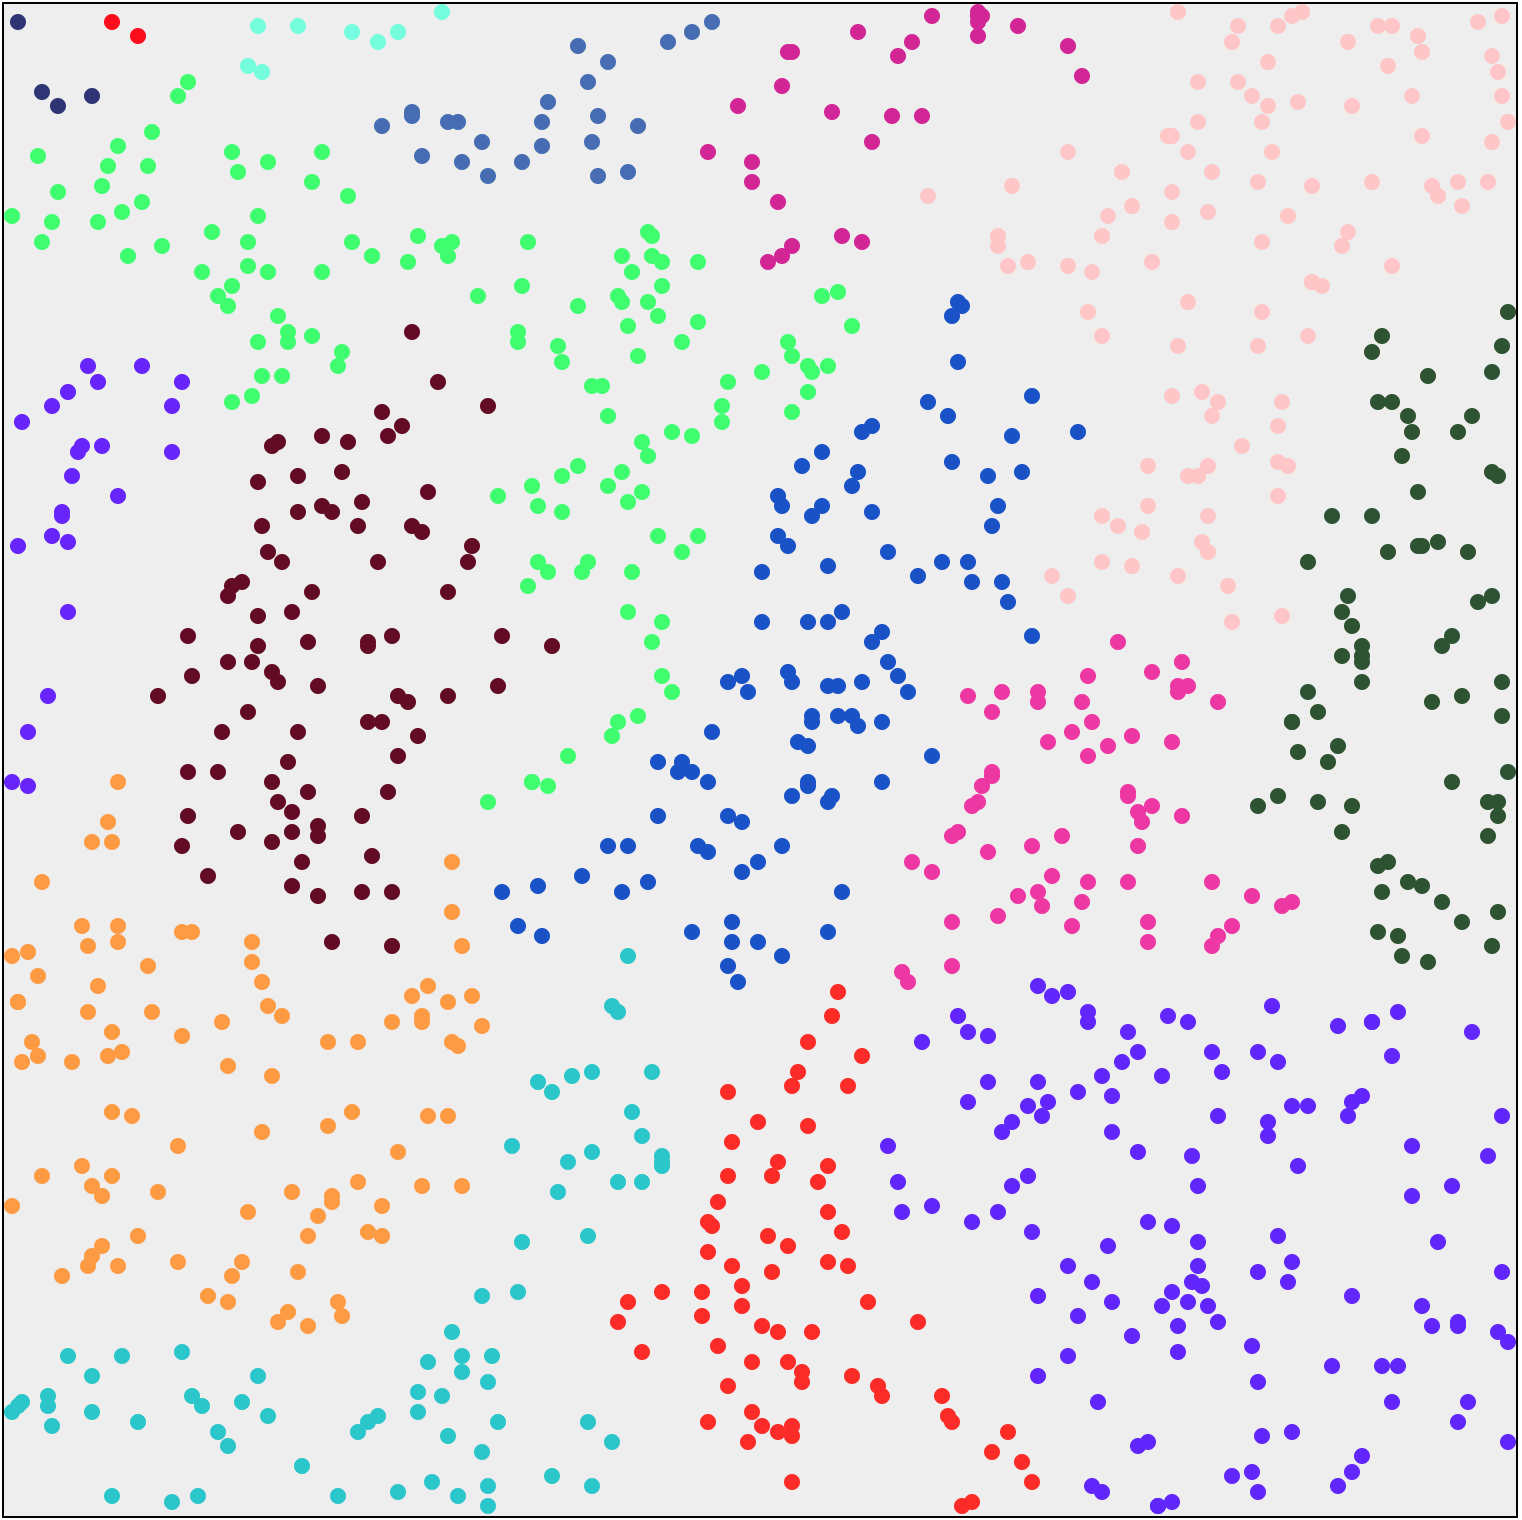
\includegraphics[width=11cm]{Images/computations/MINCUT2_UNI.png}
		\caption{Uniform distribution, 500x500, 1000 nodes}
	\end{figure}

	\begin{figure}[H]
		\centering
		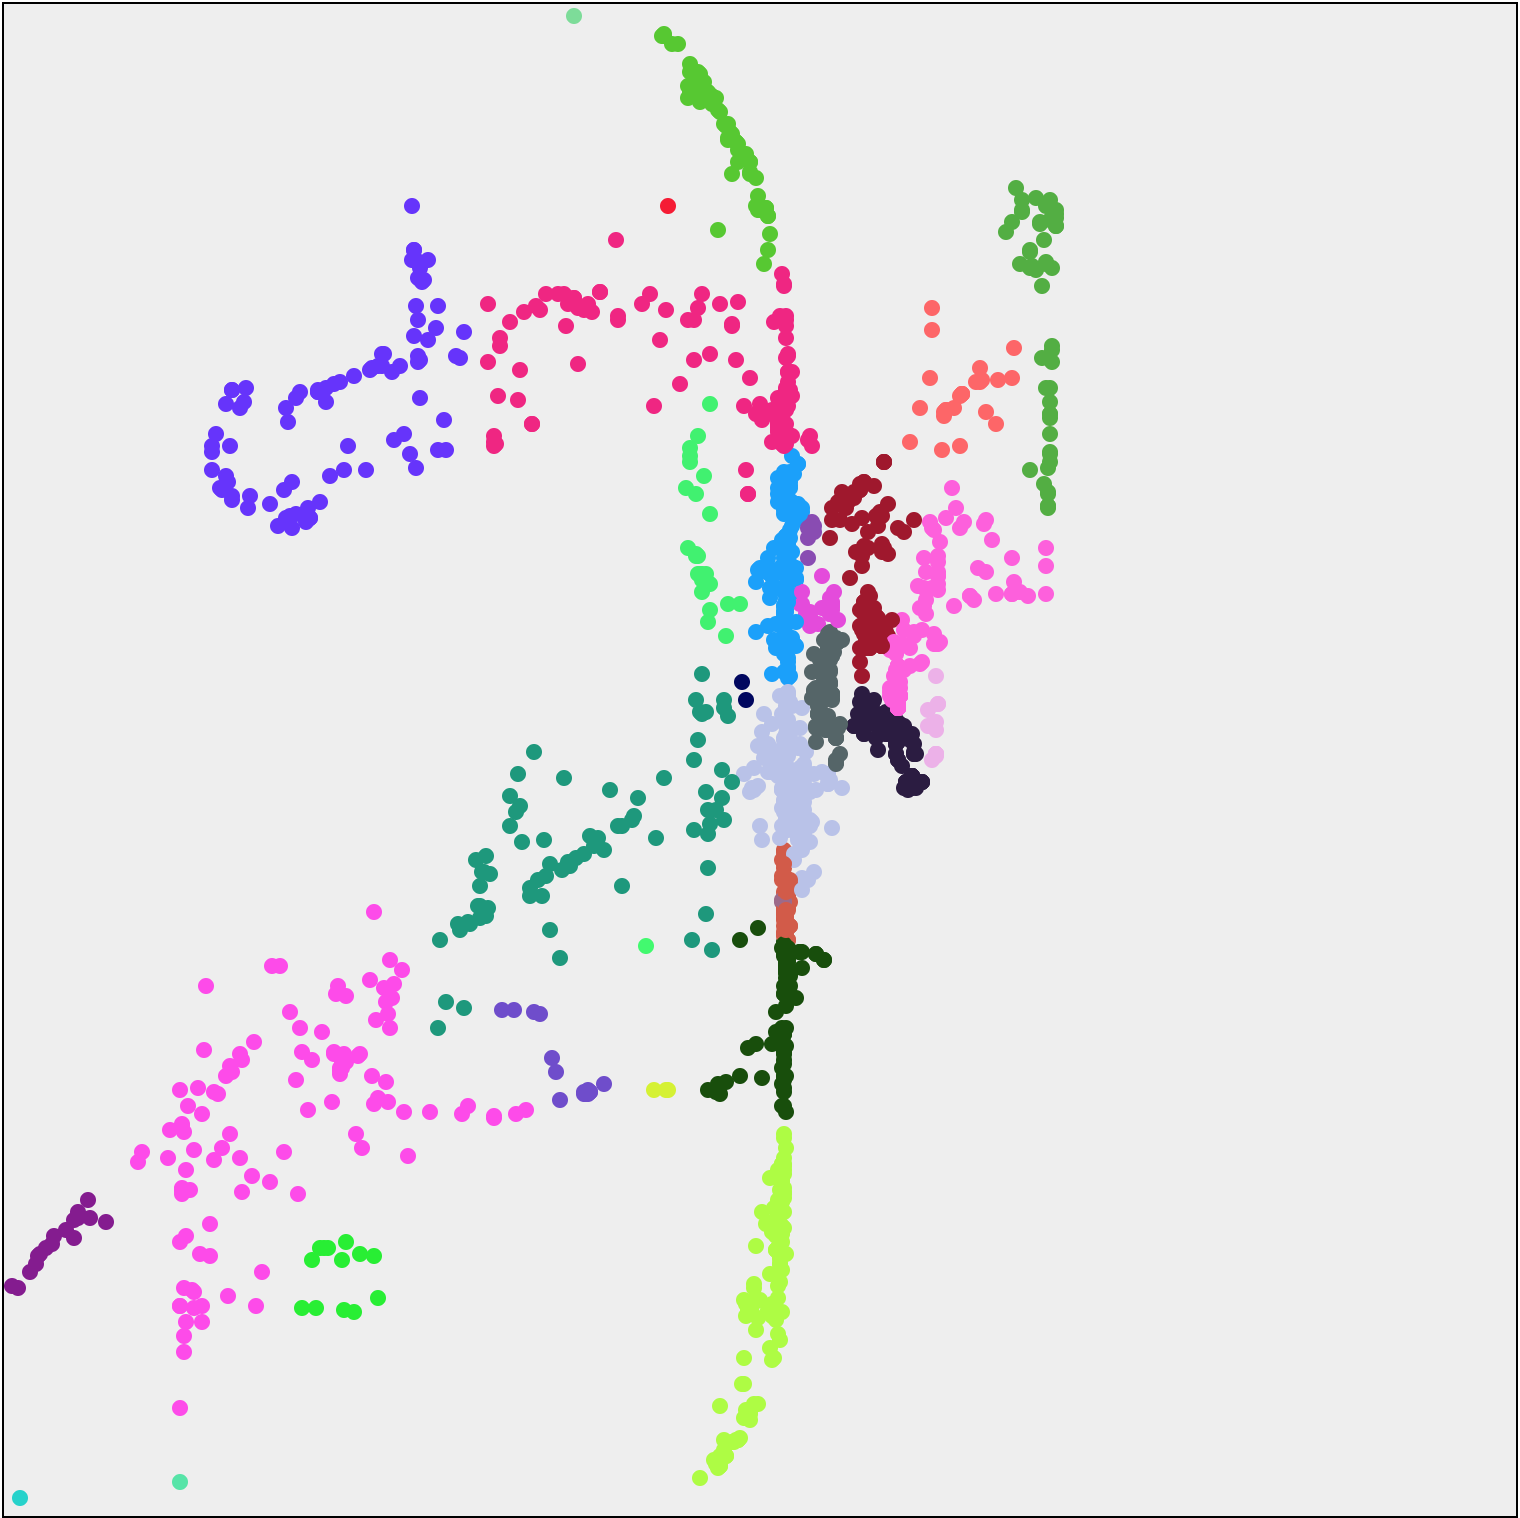
\includegraphics[width=11cm]{Images/computations/MINCUT2_FORKS.png}
		\caption{Forks, Washington, USA}
	\end{figure}

	\begin{figure}
		\centering
		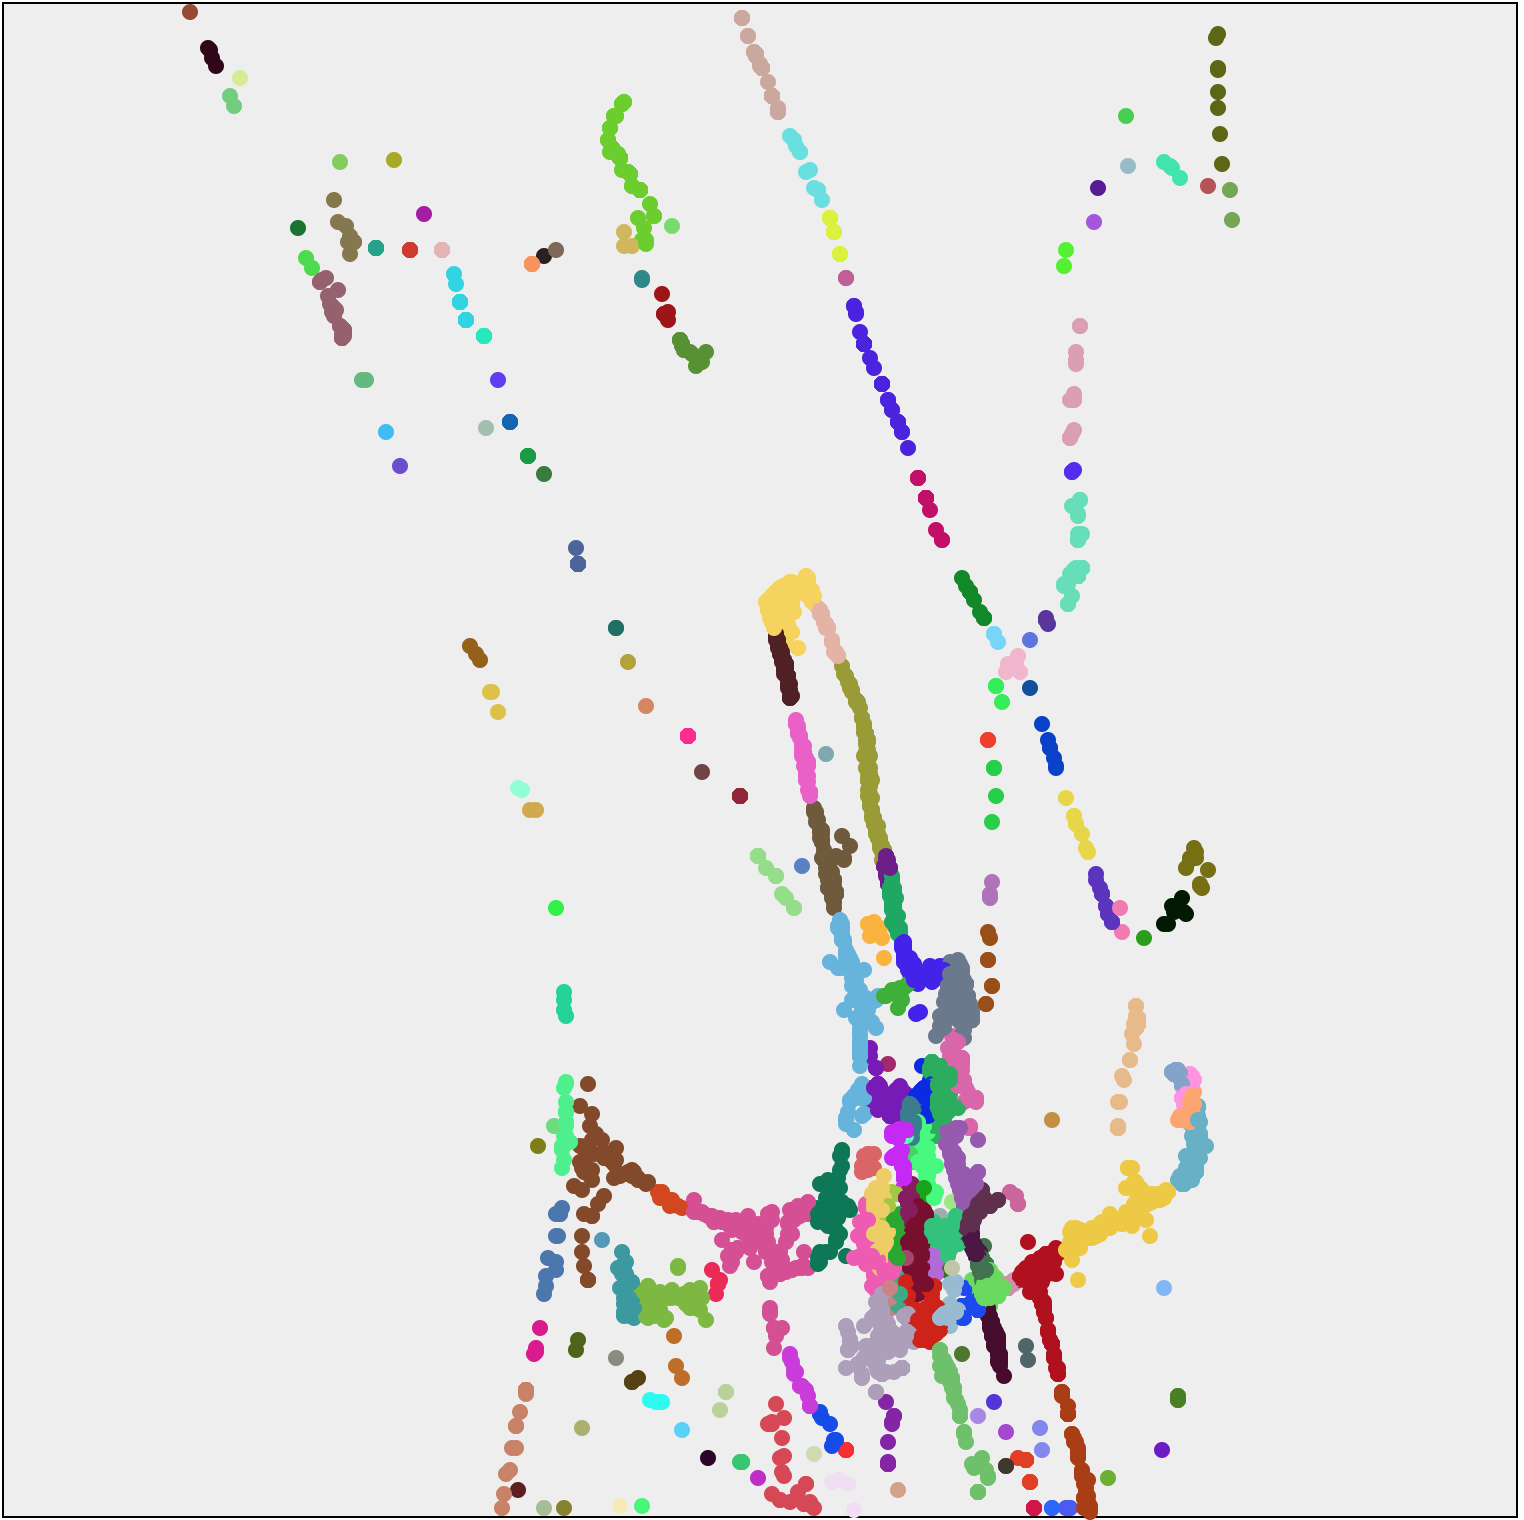
\includegraphics[width=11cm]{Images/computations/MINCUT2_LILLEHAMMER.png}
		\caption{Lillehammer, Norway}
	\end{figure}

	\begin{figure}[H]
		\centering
		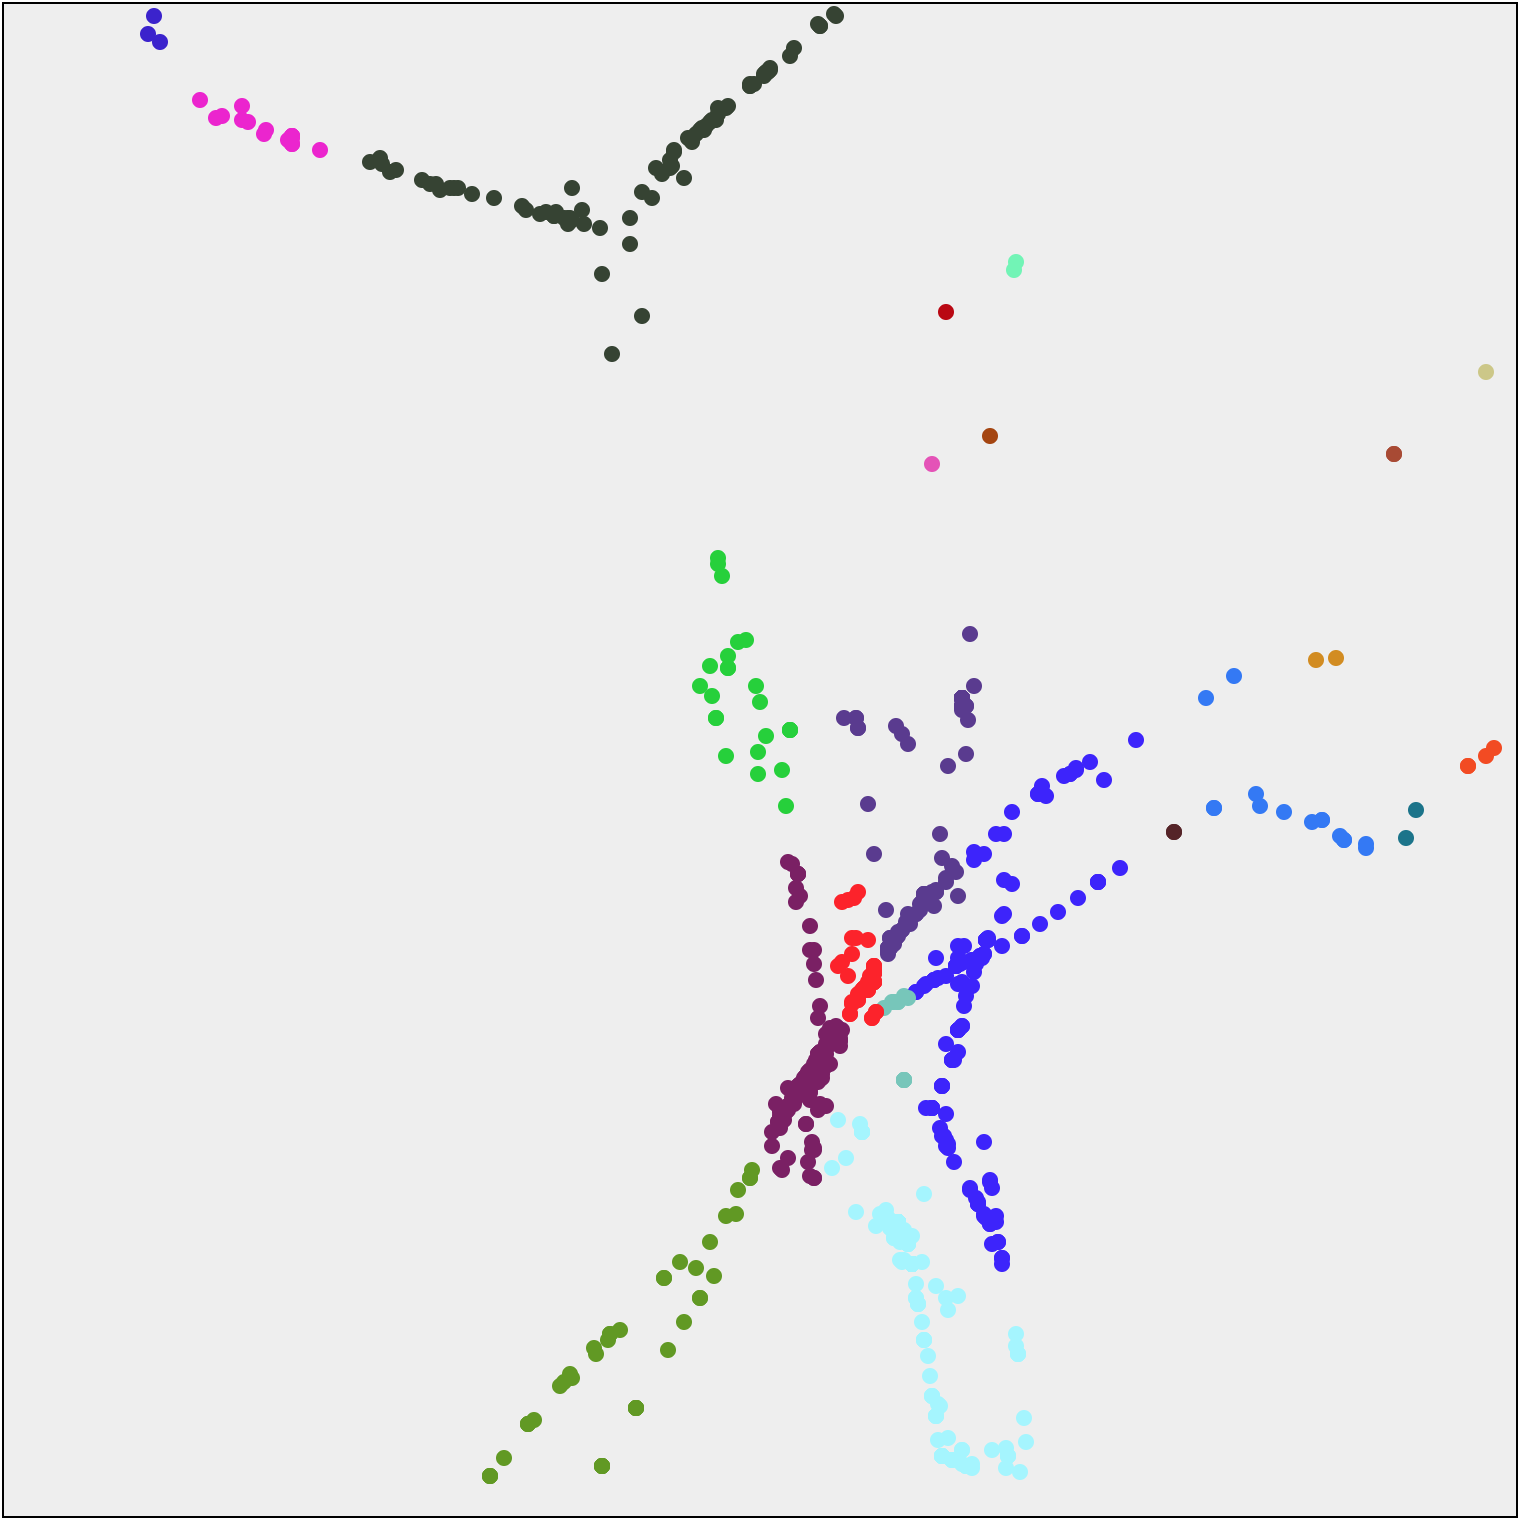
\includegraphics[width=11cm]{Images/computations/MINCUT2_TYNSET.png}
		\caption{Tynset, Norway}
	\end{figure}





\end{appendices}
